\chapter{Solução Proposta}

  Este capítulo apresenta uma visão geral da solução proposta, e se aprofunda nos projetos específicos que 
  compõem a solução final.
  
  \section{Visão geral da solução}
    
    A solução proposta conta com quatro subsistemas que se integram para compor o sistema final, são elas: 
    o sistema de captação de água, o sistema eletrônico de monitoramento e controle da qualidade da água, o sistema de 
    gestão da informação e a matriz energética.
    
    O sistema de captação de água é o responsável por produzir a água a partir da umidade do ar e conta com as turbinas para tal.
    A partir da produção da água pelas turbinas, a mesma é levada para um reservatório onde será feito todo o acompanhamento da
    qualidade da água através dos aparatos eletrônicos. No sistema de captação da água, as turbinas também contam com um monitoramento 
    feito pelos sensores de vibração da estrutura, velocidade dos ventos, temperatura das turbinas, entre outros.
    Esses dados produzidos pelos sensores serão acompanhados pelo \textit{software} de gestão da informação para permitir o controle e 
    tomada de decisões no processo de produção, por parte dos técnicos envolvidos. O sistema de gestão da informação também fará 
    o controle da distribuição da água para a população. Para dar o suporte para todo o processo de produção e acompanhamento da 
    produção, a solução possui uma matriz energética própria.
    
    \subsection{Funcionamento da turbina}
  
  O desenho esquemático da turbina apresentado na figura abaixo mostra as pás acopladas ao rotor, que por meio de um eixo cilíndrico conecta-se ao gerador. Este gerador é o responsável pela geração de energia elétrica através da energia mecânica. A energia mecânica é provinda do giro das hélices que os ventos provocam ao entrar em contato com as pás.  No compartimento à esquerda, onde se encontram o eixo do rotor e o gerador, contem também um filtro de partículas e dois cilindros de compressores. O filtro de partículas frontal é necessário para evitar que resíduos do ar danifiquem os componentes eletrônicos presentes nessa região, tendo em vista que há uma circulação de vento nesse compartimento com o âmbito de refrigerar o gerador e os compressores. Já os compressores, irão comprimir o gás presente em ductos (que estão acoplados ao condensador presente no outro compartimento) para que se atinja uma temperatura baixa possível de se realizar a condensação do ar.
  
  \FloatBarrier
  \begin{figure}[!h]
    \centering
    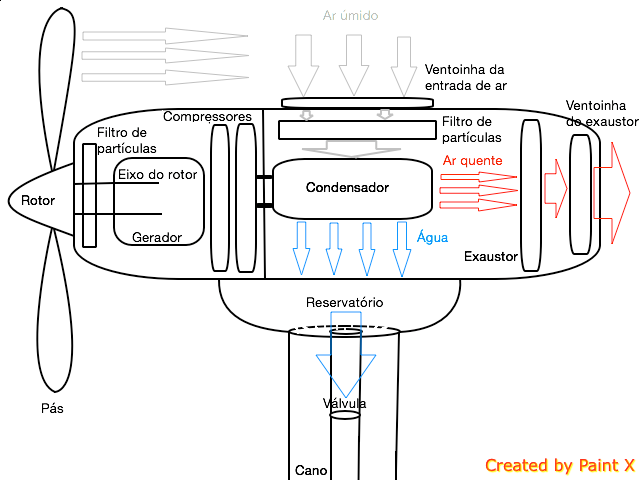
\includegraphics[scale = 0.9]{editaveis/figuras/funcionamento_turbina}
    \label{funcionamento_turbina}
    \caption[Funcionamento da turbina]{Desenho esquemático do funcionamento da turbina geradora de energia e água.}
  \end{figure}
  \FloatBarrier
    
  No segundo compartimento, que tem uma circulação de ventos independente do primeiro compartimento, estão presentes os componentes necessários para a captação de água através da umidade. A entrada de ar úmido se dá pelo topo da nacele por meio de uma ventoinha que suga o ar da atmosfera para dentro da turbina. Uma vez o ar úmido dentro da turbina, ele passa por um filtro de partículas para que as impurezas não danifiquem o funcionamento de nenhum componente. Filtrado o ar, este entra em contato com o condensador que, junto com os ductos vindos do compressor, irá condensar este ar. O ar condensado (líquido) escorre pelas paredes do condensador até cair no reservatório contido na base da nacele, enquanto o ar quente provocado pelo condensar neste processo é sugado por um exaustor e enviado diretamente para fora da nacele por meio de uma ventoinha presente no extremo oposto às pás. A água permanece no reservatório até que sensores permitam a abertura da válvula de escoamento que, uma vez aberta, toda a quantidade de líquido até então armazenada escorrerá, por ação da gravidade, pelo cano presente ao longo da torre de sustentação.
  O monitoramento do estado das turbinas será feito pelo sistema de gestão da informação com os dados obtidos pelos sensores na estrutura 
  da turbina.

\subsection{Monitoramento eletrônico e adição de sais}

  \begin{figure}[!htbp]
    \centering
    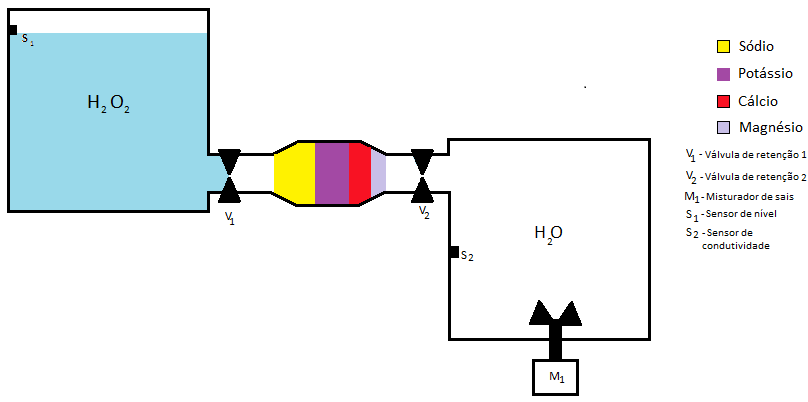
\includegraphics[scale=0.6]{editaveis/figuras/sistema_adicionador_sais}
    \caption[Esquemático do sistema adicionador de sais]{Esquemático do sistema adicionador de sais.}
    \label{sistema_adicionador_sais_1}
  \end{figure}
  \FloatBarrier
    
Após sair da turbina, a água irá descer pelo cano em direção ao reservatório. A água provinda da turbina contará com processos
mecânicos e digitais, sendo assim, após filtragem a água é direcionada para o tanque primário, o qual encherá até certo nível.
A água passará então por um filtro que adicionára os sais necessário à agua, jogando a àgua adicionada de sais em outro tanque,
onde há um misturador para realizar a solubilização dos sais na água.

Nestes reservatórios também se encontram os sensores necessários para o monitoramento da qualidade da água e dos níveis do reservatório.


\subsection{Monitoramento do sistema de gestão da informação}

  O controle de tais sensores se dará por meio do software, cuja finalidade principal é o monitoramento do sistema como um todo. Nele haverá informações relacionadas à qualidade e quantidade da água obtida, características do ambiente externo onde as turbinas se encontram casa de controle, distribuição de energia excedida, ao armazenamento e tratamento com sais da água ainda dados sobre a turbina.
	 
  Alguns dos dados referentes à turbina que serão monitorados pelo software são: as temperaturas internas, a quantidade de energia gerada por cada turbina, a velocidade de rotação das pás. A qualidade da água também será monitorada, pois o software fará as devidas leituras dos sensores, dados relacionados à casa de controle incluem, por exemplo, a voltagem das baterias, a falta ou presença de energia. Com relação à distribuição de energia, o software deve mostrar se a energia excedida está sendo direcionada a rede ou se está abastecendo a casa de controle.

  Também serão obtidos dados referentes à umidade do ar e as características do vento de onde as turbinas se encontram, como exemplo de dados relacionados ao ambiente externo. Percebe-se, portanto, que o software que será utilizado possibilitará o monitoramento de uma série de aspectos relacionados a tecnologia de captação de água a partir da umidade do ar.

  Além de realizar a manutenção da água, e os sensores que capacitam a boa qualidade da água distribuída, os softwares permitirão o cadastro de pessoas que chegarão para buscar a água. Isso permite que façamos um censo e adequemos o sistema a cada mudança de demanda por água, seja por que o número de pessoas atendidas tenha aumentado ou diminuído.

\subsection{Distribuição da água}
  A água será distribuída através de torneiras acopladas a parte externa da torre de controle, com acesso direto ao produto final. A água que ficar em excesso no reservatório será engarrafada em garrafas apropriadamente higienizadas, as quais serão cedidas pelas empresas parceiras. Sendo essas também responsáveis pelo destino das garrafas quando chegar a hora do descarte delas.
  
  \FloatBarrier
  \begin{figure}[!h]
      \centering
      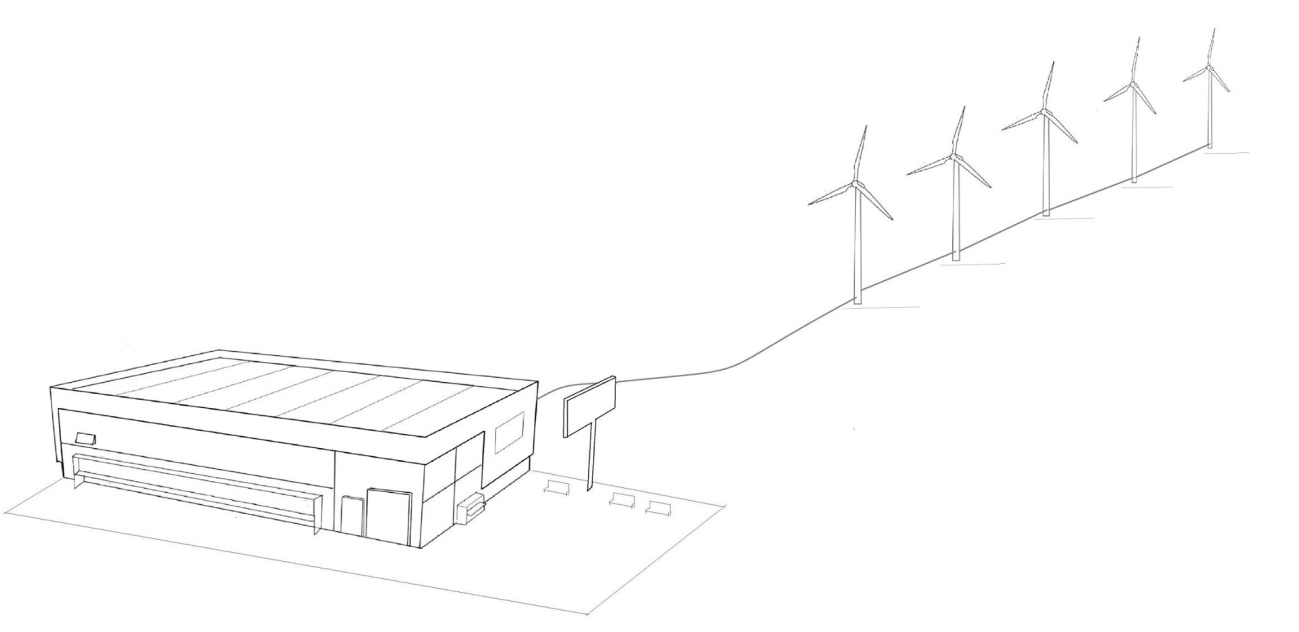
\includegraphics[scale = 0.4]{editaveis/figuras/distribuicao_agua}
      \label{distribuicao_agua}
      \caption[Distribuição água]{Esquema de distribuição da água até chegar ao local de distribuição.}
  \end{figure}
  \FloatBarrier
  
  A prefeitura Municipal de Acari, juntamente com empresas parceiras construirá uma praça de finalidade educacional da população, onde será localizado o centro de distribuição de água. A água será distribuída de forma gratuita, pois o projeto visa o lado social e a melhora na qualidade de vida.



  \section{Sistema de captação de água}
    
      Para condensar o vapor de água presente no ar, usaremos do conceito de temperatura de orvalho. A temperatura de orvalho 
      é a temperatura na qual o ar começa a se condensar, pois sua umidade relativa chega a 100\%. Foi feita uma estimativa
      teórica da produção de água pela turbina. O cálculo se encontra no anexo \ref{estimativa_producao_agua}.
      
      O funcionamento do sistema de captação de água se dá da seguinte maneira: primeiro, captamos o ar úmido e quente do ambiente.
      Em seguida, abaixamos a temperatura do ar até abaixo da temperatura de orvalho. O ar não suportará toda a umidade que ele
      conterá, e desprenderá parte dela. Essa parte de vapor de água condensado é a água que coletaremos em nossa turbina. 
      Para resfriar essa massa de ar, usaremos um ciclo de refrigeração composto de compressores , evaporador e condensador,
      que será abordado no tópico seguinte.
    
    \subsection{Peças da turbina}
      
      Esta seção apresenta as peças definidas para composição das turbinas do sistema de captação de água.
      
    	\subsubsection{Compressor}
		Em um sistema de refrigeração, há vários processos operados por vários maquinários, equipamentos e válvulas. Um desses equipamentos é o compressor que tem a função de receber um determinado gás a baixa temperatura e pressão e aumentar a pressão e, consequentemente, a temperatura. Esse processo pode ser esquematizado pela figura abaixo, onde o compressor está indicado pelo círculo amarelo.
\begin{figure}[!htbp]
  \centering
  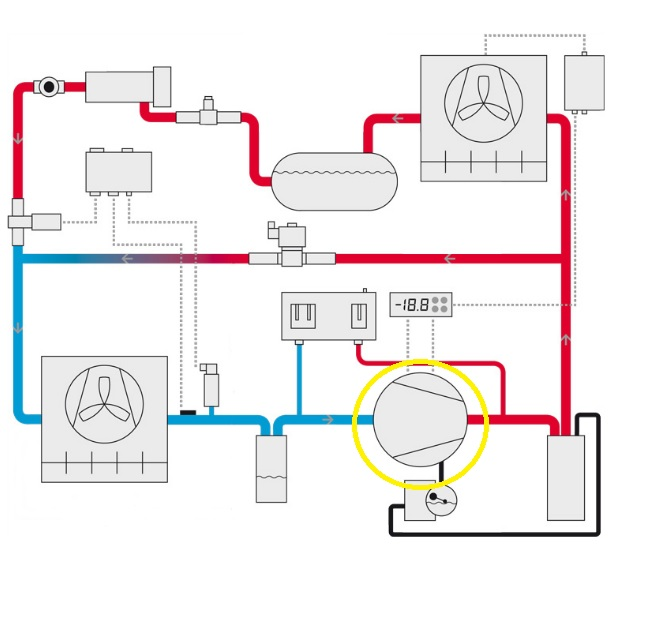
\includegraphics[scale=0.6]{editaveis/figuras/compressor}
  \caption[Esquematização processo refrigeração]
  {Esquematização de um processo de refrigeração. O compressor se localiza no circulo amarelo.\footnotemark}
  \label{compressor}
\end{figure}
\footnotetext{Fonte:Emerson Technologies}
\FloatBarrier
Analisando como base a turbina WMS1000 Wind Turbine da Eolewater, percebe-se que dentre os inúmeros tipos de compressores existentes, o compressor do tipo espiral (Scroll Compressor) é o melhor e mais recomendado, principalmente pela sua capacidade de operação  e pelo seu tamanho reduzido, que é essencial visto que o espaço é muito limitado dentro turbina. Ele também pode ser combinado com outros compressores para dar ao sistema uma maior eficiência e capacidade\cite{compressors}.

Após a escolha do tipo de compressor, deve-se analisar entre os vários tipos de configuração de um compressor espiral pode ter e escolher um que adeque aos requisitos do projeto. Tomando como base a WMS1000, um compressor de aproximadamente 15KW  deverá ser usado em duplicidade para o sistema de refrigeração. 

A empresa escolhida para ser a fornecedora desse compressor foi a Emerson Electric Company, que tem tradição e tecnologia de ponta nessa área. Será usada a série de compressores Copeland Scroll™.  Essa escolha foi feita através da análise das características de cada modelo dado pela empresa como mostra a foto abaixo. Como a expectativa era de que o compressor tivesse uma potência de 15KW, e não dispondo desse modelo na empresa, foi escolhido o modelo digital ZBD 76KCE-TFD, que tem um pequeno acréscimo de potência, tornando-o o mais adequado. 

\textit{Copeland Scroll Digital Model Overview}

	\begin{figure}[!htbp]
	  \centering
	  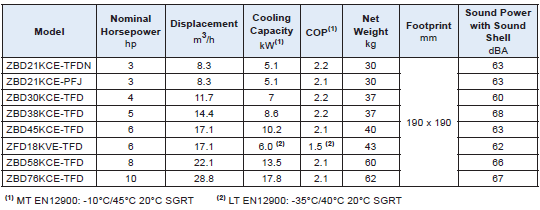
\includegraphics[scale=0.5]{editaveis/figuras/tabela_compressores}
	  \caption[Modelos de compressores]{Tabela com modelos de compressores da EmersonTM e suas características principais.\footnotemark}
	  \label{tabela_compressores}
	\end{figure}
	\footnotetext{Fonte:Emerson Technologies}
	\FloatBarrier
A EmersonTM disponibiliza seus compressores com vários tipos de líquidos refrigerantes, mais deve-se trabalhar com os materiais que possam ter o mínimo de impacto negativo na natureza. 


	\begin{figure}[!htbp]
	  \centering
	  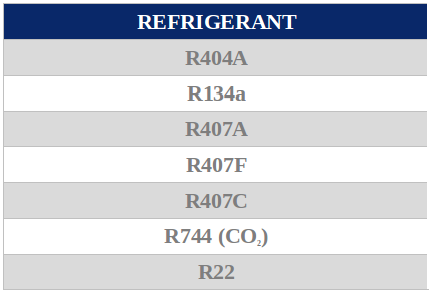
\includegraphics[scale=0.4]{editaveis/figuras/tabela_gases_refrigerantes}
	  \caption[Gases refrigerantes]{Gases refrigerantes disponibilizados pela Emerson em seus compressores.\footnotemark}
	  \label{gases_compressores}
	\end{figure}
	\footnotetext{Fonte:Emerson Technologies}
\FloatBarrier
Analisando os tipos de refrigerantes, o melhor que se poderia usar, levando em consideração seus impactos ambientais, seria o R-410A. O R-410A é um gás com efeito inofensivo a camada de ozônio, mais não ao aquecimento global \cite{essencials_r410A}. Como a EmersonTM não disponibiliza tal gás refrigerante, a escolha mais apropriada será o R-407C, que é  um substituto do R-22, um gás largamente usado e de alto impacto na camada de ozônio e no aquecimento global \cite{epa2014}. 

O R-407C vem sendo utilizado na substituição do R-22, pois o R-410A não pode ser o substituo do R-22 por causa do alto nível de pressão em que trabalha os compressores \cite{epa2014}. Mas a EmersonTM não disponibiliza o R-407C para o modelo selecionado de compressor, por isso, decidiu-se utilizar o R-407A no compressor do projeto, ainda assegurando um requisito ambiental e operacional. 

Assim, para o líquido refrigerante R407-A, o compressor espiral de modulação terá as seguintes características gerias de operação: 

	\begin{figure}[!htbp]
	  \centering
	  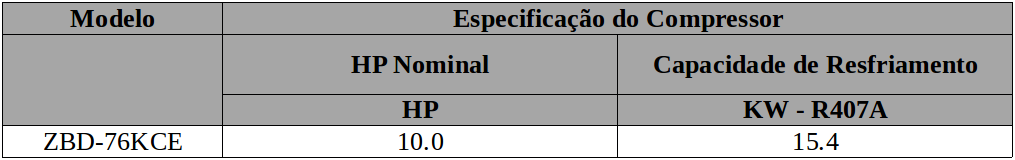
\includegraphics[scale=0.4]{editaveis/figuras/tabela_especificacao_compressor}
	  \caption[Especificação Compressor]{Características gerais do compressor.\footnotemark}
	  \label{gases_compressores}
	\end{figure}
	\footnotetext{Fonte:Emerson Technologies}
	\FloatBarrier
Abaixo segue várias informações do fabricante sobre o Compressor modelo ZBD-76KCE:

	\begin{itemize}
	 \item Características Gerais:
	 
	\begin{figure}[!htbp]
	  \centering
	  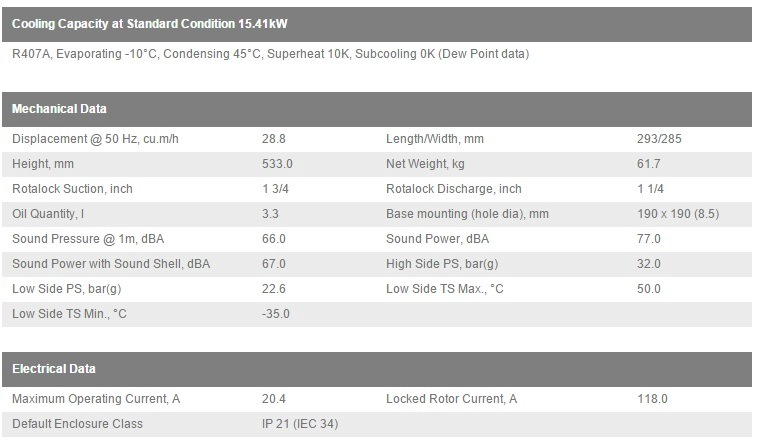
\includegraphics[scale=0.7]{editaveis/figuras/tabela_cooling_capacity}
	  \caption[Capacidade de cooling]{Características gerais do compressor.\footnotemark}
	  \label{tabela_cooling_capacity}
	\end{figure}
	\footnotetext{Fonte:Emerson Technologies}	   
	 \FloatBarrier
	 \item Envelope de Operação:  
	 
	\begin{figure}[!htbp] 
	  \centering
	  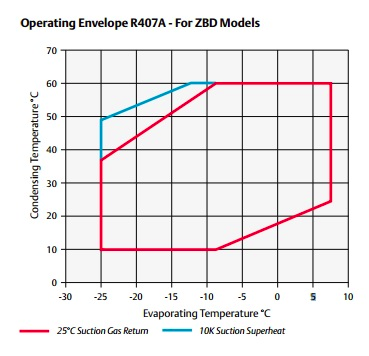
\includegraphics[scale=0.6]{editaveis/figuras/grafico_opereting_envelope}
	  \caption[Envelope de operação]{Envelope de operação.\footnotemark}
	  \label{grafico_opereting_envelope}
	\end{figure}	
	\footnotetext{Fonte:Emerson Technologies}   
	\FloatBarrier
	 \item Dimensões: 
	 
	\begin{figure}[!htbp] 
	 \centering
	  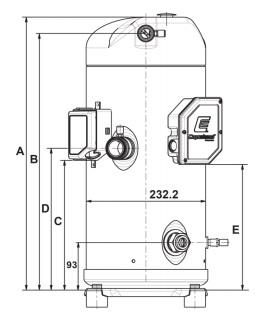
\includegraphics[scale=0.7]{editaveis/figuras/dimensao_compressor}
	  \caption[Dimensões]{Dimensões\footnotemark}
	  \label{grafico_opereting_envelope}
	\end{figure}	   
	\footnotetext{Fonte:Emerson Technologies}
	\FloatBarrier
	\begin{figure}[!htbp]
	 \centering
	  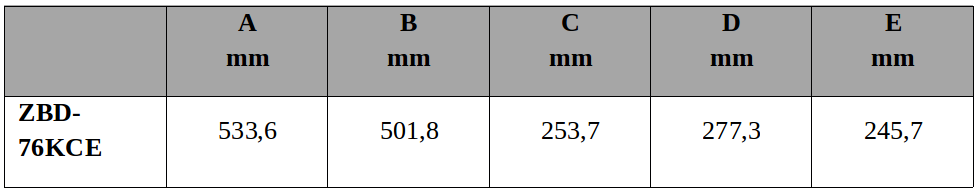
\includegraphics[scale=0.4]{editaveis/figuras/dimensao_compressor_2}
	  \caption[Dimensão compressor]{Dimensões\footnotemark}
	  \label{grafico_opereting_envelope}
	\end{figure}	   
	\footnotetext{Fonte:Emerson Technologies}
	\FloatBarrier
	\end{itemize}	
	\subsubsection{Valvula expansora}
		Sabendo-se que o sistema de refrigeração tem a parte de alta temperatura e o de baixa, é necessário entender quem são os intermediários entre essas duas partes. Da baixa temperatura e pressão para alta temperatura e pressão, está o compressor. Já para intermediar o líquido refrigerante quente do gás gelado, temos a válvula de expansão. 

O funcionamento de uma válvula de pressão tem por finalidade reduzir a pressão do refrigerante e controlar o fluxo de massa que entrará no evaporador. Assim sendo, ele é essencial para um funcionamento perfeito, visto que ele deve manter um superaquecimento constante para evitar que o haja a entrada de líquido no compressor. 

Para a escolha específica da válvula, deverá ser analisado todo o conjunto do sistema para uma melhor determinação das especificações do produto. Analisando a nomenclatura, já se pode dizer que será usado uma válvula de equalização de pressão externa, visto que são comumente usados para sistemas mais robustos e que demandam grande quantidade de liquido refrigerante pelo sistema\cite{compressors_for_refrigeration}. 

Além disso, a escolha de uma válvula está ligada ao compressor, visto que, se escolhermos um circuito dotado de tubos capilares, as pressões antes e depois são iguais mesmo quando o compressor é desligado, isto da chance de ter um motor com baixo torque de partida. Já um circuito com válvula de expansão terá suas pressões iguais somente quando o compressor estiver ligado, requerendo um motor com alto torque de partida\cite{embracovalvula}. 

Não definiu-se ainda o fabricante da peça, visto que há vários fornecedores estrangeiros, como a Emerson Climate Technology ou a Danfoss, ou fornecedores nacionais como a Embraco. A média de preço de uma válvula do tipo de pressão externa varia entre R\$ 100,00 a R\$ 350,00.
    
	\subsubsection{Condensador}
		A refrigeração é definida como qualquer processo que vise transferir continuamente a energia térmica de uma região de baixa temperatura para uma de maior temperatura.No nosso caso, condensadores são  trocadores de calor onde o refrigerante vem do compressor a alta pressão e temperatura, troca calor com a água ou ar mudando de estado, passando de vapor para líquido-condensado. 

O tamanho requerido e a configuração de um condensador são baseados na temperatura saturada de condensação da aplicação.Além de procurar trabalhar com temperaturas de condensação baixas visando aumentar a eficiência do sistema, o projeto final do condensador deve resultar em uma unidade que é um equilíbrio entre a praticidade e a economia.

Condensadores resfriados a ar são disponíveis em uma variedade de configurações e capacidades que variam de 3,5 kW a 351,7 kW. Devido o calor específico do ar ser relativamente pequeno, é necessário uma grande quantidade de ar por unidade de transferência de calor. Esta característica restringe o tamanho de condensadores resfriados a ar, em recinto fechado ou localizados ao ar livre para capacidades menores. 

O melhor condensador levando em conta a torre de captação,e a turbina eólica, com aproveitamento gravitacional do terreno aplicado seria o, Condensador vertical com condensação na carcaça e retorno do refluxo sob ação da gravidade.
	\begin{figure}[!htbp]
	 \centering
	  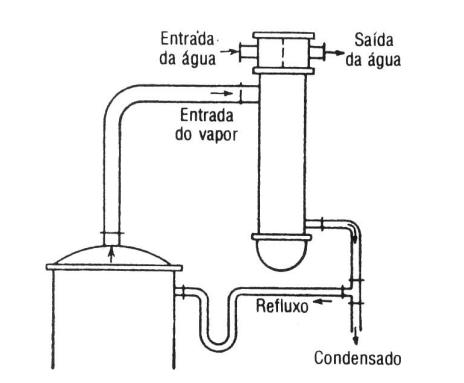
\includegraphics[scale=0.4]{editaveis/figuras/condensador}
	  \caption[Condensador]{Condensador\footnotemark}
	  \label{condensador}
	\end{figure}	   
	\footnotetext{Disponível em: http://www.essel.com.br/cursos/material/03/Ap12.pdf}
	\FloatBarrier
	\begin{figure}[!htbp]
	 \centering
	  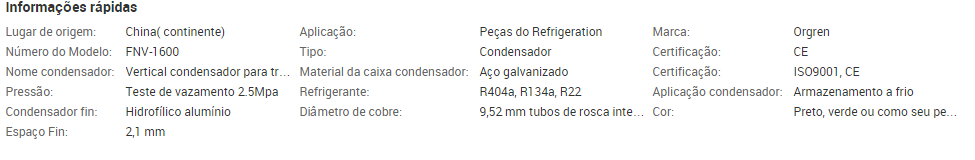
\includegraphics[scale=0.4]{editaveis/figuras/informacao_condensador}
	  \caption[Informações sobre o condensador]{Informações sobre o condensador\footnotemark}
	  \label{condensador_informacao_1}
	\end{figure}	
	\footnotetext{Disponível em:http://portuguese.alibaba.com/product-gs/vertical-condenser-for-heat-exchange-60225996798.html}   
	\FloatBarrier	
	\begin{figure}[!htbp]
	 \centering
	  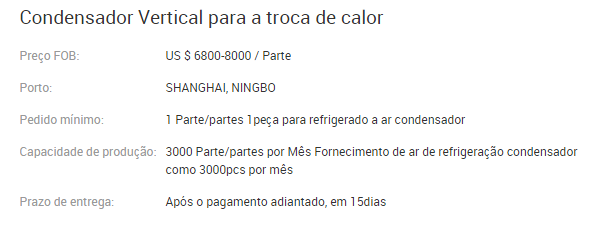
\includegraphics[scale=0.4]{editaveis/figuras/condensador_vertical}
	  \caption[Informações sobre o condensador 2]{Informações sobre o condensador\footnotemark}
	  \label{condensador_informacao_2}
	  \footnotetext{Disponível em: http://portuguese.alibaba.com/product-gs/vertical-condenser-for-heat-exchange-60225996798.html }
	\end{figure}
		\FloatBarrier
	\subsubsection{Evaporador}
		No sistema de refrigeração, o evaporador é a parte onde o resfriamento do meio ocorre. Isso se dá pelo processo em que o refrigerante, na forma líquida, ao passar por essa região, absorve o calor do meio e assim evapora transformando-se em gás novamente. 
\begin{figure}[!htbp]
	 \centering
	  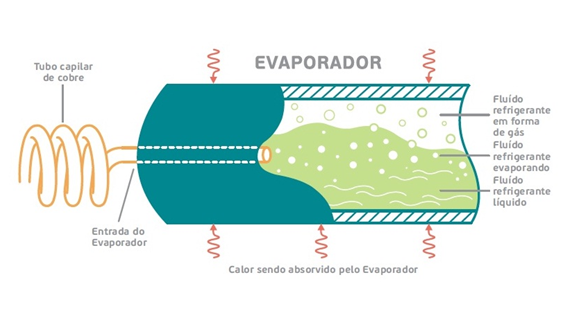
\includegraphics[scale=1]{editaveis/figuras/evaporador}
	  \caption[Esquema de processo de evaporação de o refrigerante]{Esquema de processo de evaporação de o refrigerante\footnotemark}
	  \label{condensador}
	\end{figure}	   
	\footnotetext{Disponível em: http://www.clubedarefrigeracao.com.br/material/colecao-tecnica}
	\FloatBarrier
	
	
Basicamente, existem alguns tipos de evaporadores e eles variam de acordo com a disposição ou necessidade. O evaporador de do tipo placa (roll-bond) é muito comum nas casas brasileiras, já que pode ser encontrado nos refrigeradores domésticos. Ele é composto por duas chapas de alumínio sobrepostas e entre elas um tubulação em forma de ziguezague por onde passa o refrigerante. Outro tipo bem parecido é o tubular, que apresenta uma serpentina colada em uma placa de alumínio.\cite{embracocolecao}.

O evaporador aletado apresenta um tubo de alumínio com aletas de alumínio \cite{embracocolecao}. Diferente dos dois tipos apresentados no paragrafo anterior, esse aveporador, tambem chamado de evaporador de ar forçado, precisa de um ventilador que possa movimentar o ar para dentro e assim ter uma maior vazão. 

Com essa análise, foi escolhido o evaporador de ar forçado, visto que, em caso de haver pouco vento ou variação do mesmo na região de Acarí, a produção de água não seria prejudicada já que os ventiladores serviram para manter um fluxo constante de entrada de ar para que a produção de água fique dentro das metas já pré-estabelecidas. 
Outra justificativa para escolha desse tipo de evaporador é que ele se adequa as restrições feitas pelos cálculos no Anexo A, que definem a vazão necessária para que ocorra a produção da quantidade de água prevista pelo escopo.

O fabricante do evaporador escolhido foi a TrinevaTM, principalmente porque eles trabalham com evaporadores de alta vazão e, por ser um fabricante nacional, tornará o custo do produto e do frete mais acessíveis em relação à um fabricante no exterior. 

\begin{figure}[!htbp]
	 \centering
	  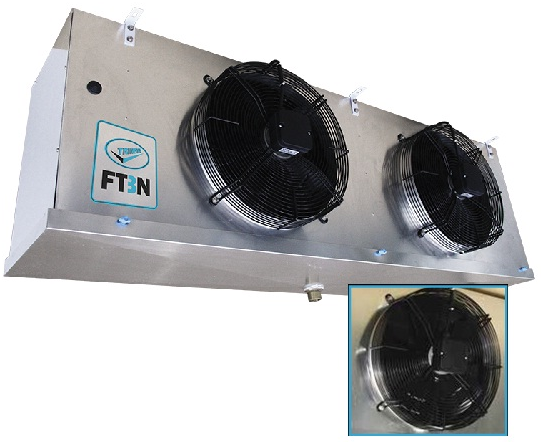
\includegraphics[scale=1]{editaveis/figuras/evaporador_trivena}
	  \caption[Evaporador trivena]{Evaporador Trineva\textsuperscript{TM} da linha FTBN e, em detalhe, o motoventilador de 400mm com rotor externo \footnotemark}
	  \label{evaporador}
	\end{figure}	   
	\footnotetext{Disponível em: http://trineva.com.br/?page\_id=122}
	\FloatBarrier
	
Essas dimensões apresentadas podem ser atribuídas as seguintes cotas da imagem abaixo.
\begin{figure}[!htbp]
	 \centering
	  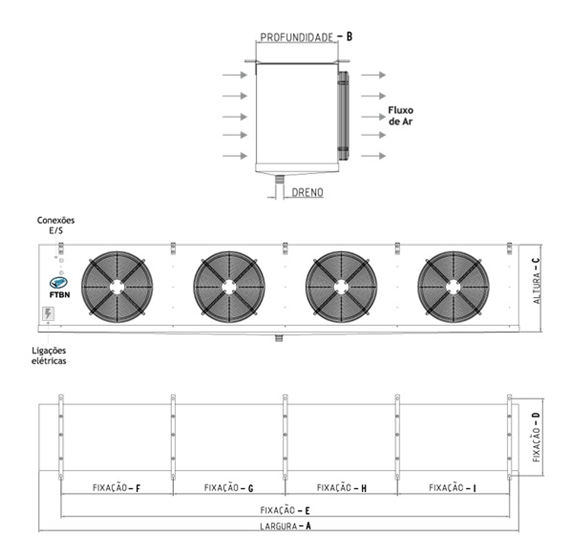
\includegraphics[scale=1]{editaveis/figuras/cotas_evaporador}
	  \caption[Cotas evaporador]{Cotas das três vistas ortográficas do modelo geral de evaporador \footnotemark}
	  \label{cota_evaporador}
	\end{figure}	   
	\footnotetext{Disponível em: http://trineva.com.br/?page\_id=122}
	\FloatBarrier
	
O desempenho térmico e a vazão do evaporador escolhido estão dentro do quadro amarelo da imagem que se segue.
\begin{figure}[!htbp]
	 \centering
	  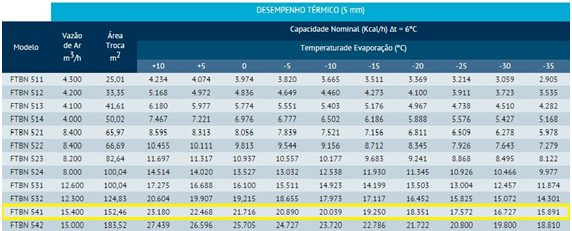
\includegraphics[scale=1]{editaveis/figuras/desenho_termico}
	  \caption[Vazão do evaporador]{Vazão do evaporador, assim como sua área e desempenho térmico \footnotemark}
	  \label{vazao_evaporador}
	\end{figure}	   
	\footnotetext{Disponível em: http://trineva.com.br/?page\_id=122}
	\FloatBarrier
	
Para os ventiladores e o sistema de degelo, a Trineva\textsuperscript{TM} fornece os seguintes dados para o modelo escolhido:
\begin{figure}[!htbp]
	 \centering
	  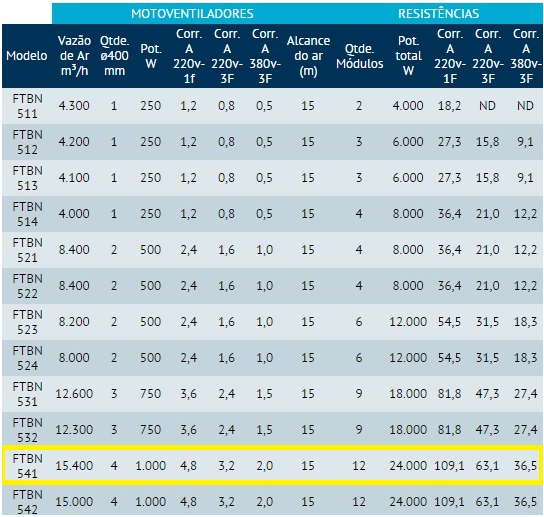
\includegraphics[scale=1]{editaveis/figuras/dados_ventiladores}
	  \caption[Dados dos ventiladores]{Dados dos ventiladores e das resistências elétricas \footnotemark}
	  \label{vazao_evaporador}
	\end{figure}	   
	\footnotetext{Disponível em: http://trineva.com.br/?page\_id=122}
	\FloatBarrier
	\subsubsection{Filtro de Partículas de Ar}
		 O  filtro de ar escolhido foi o Filtro de partículas de ar de alta performance (HEPA), que possui em sua composição fibra de vidro  e outros materiais, arranjados aleatoriamente, formando uma espécie de teia capaz de filtrar partículas indesejadas. Essas partículas passam e aderem as fribras pelos seguintes mecanismos: \cite{edge}
    
	\begin{enumerate}
	 \item Interceptor: responsável por direcionar as partículas para as fibras.
	 \item Impacto: gera o impacto direto das partículas maiores com a fibra.
	 \item 3. Difusão : partículas com menos de 0,1 mícrons tem maior probabilidade de passar sem serem aderidas pelas fibras, então elas colidem com um gás que as fazem movimentar possibilitando a aderência pela fibra.
	\end{enumerate}
	 
Informações:\cite{filtracom}

	\begin{itemize}
	 \item Possui eficiência mínima de 99,97\% para partículas de 0,3 mícrons;
	 \item Comercializado no Brasil, principalmente, pelas empresas Filtracom e Aeroglass;
	 \item Classes de filtragem: H11, H12, H13, H14 e U15, que atendem as normas europeias EN779, EN1822 e as brasileiras A1 e A3 da ABNT.
	\end{itemize}
	
	\begin{figure}[!htbp]
	 \centering
	  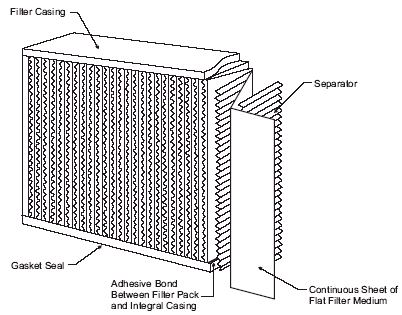
\includegraphics[scale=0.5]{editaveis/figuras/filtro_ar}
	  \caption[Imagem do filtro de ar]{Imagem do filtro de ar\footnotemark}
	  \label{filtro_ar}
	\end{figure}
	\footnotetext{Disponível em: http://www.engineersedge.com/filtration/hepa\_filter.htm }
	\subsubsection{Controle do fluxo de ar interno}
		O projeto da Eole Water não fornece todos os dados de especificação da ventoinha que está localizada aproximadamente no centro do topo da torre eólica, nem ao fundo. A única informação possível de ser adotado foi a taxa de fluxo de ar que passa pela ventoinha original, o qual é de 30000 $m^3$/h. 
	Com tal parâmetro a ventoinha foi escolhida:
	Modelos: DQ 1000-8 ou DR 1000-8  da fabricante Rosenberg\cite{axair}
	
	\begin{itemize}
		
		\item Ambas possuem um diâmetro de 1000 mm de ventoinha e 1170 de suporte lateral, com proteção de grade na entrada da ventoinha. Possuem largura de no máximo 330 mm;
		\item O peso varia de 74 a 70 kg;
		\item Voltagem de 280 V a 400 V para se adequar aos 30000 $m^3$/h necessários;
		\item Frequência de 50Hz;
		\item Temperatura de operação $45\,^{\circ}\mathrm{C}$,;
		\item Potência de 2,15 kW;
		\item Velocidade de 8,9 m/s a 10 m/s.		
	\end{itemize}
	
Estrutura:

	\begin{figure}[!htbp]
	 \centering
	  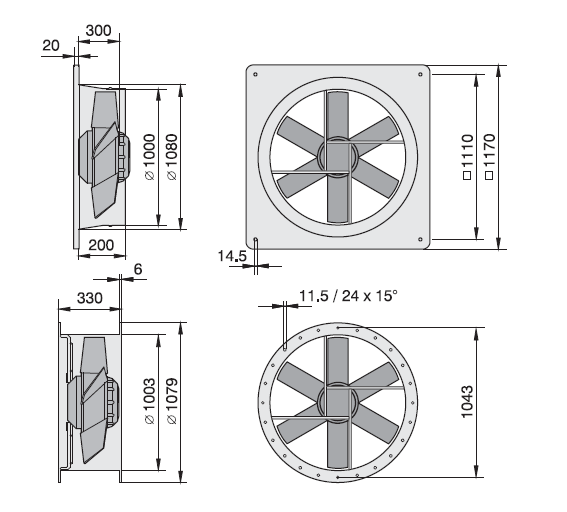
\includegraphics[scale=0.5]{editaveis/figuras/estrutura_ventoinha}
	  \caption[Imagem da estrutura da ventoinha]{Imagem da estrutura da ventoinha\footnotemark}
	  \label{estrutura_ventoinha}
	\end{figure}
	\FloatBarrier
	\footnotetext{Disponível em: http://www.axair-fans.co.uk/assets/product-resources/download/Axair\%20Fans\%20-\%20Rosenberg\%20Selection\%202013.pdf}
	
Grafico de Pressão, Fluxo de ar e Tensão de ambos os modelos:

	\begin{figure}[!htbp]
	 \centering
	  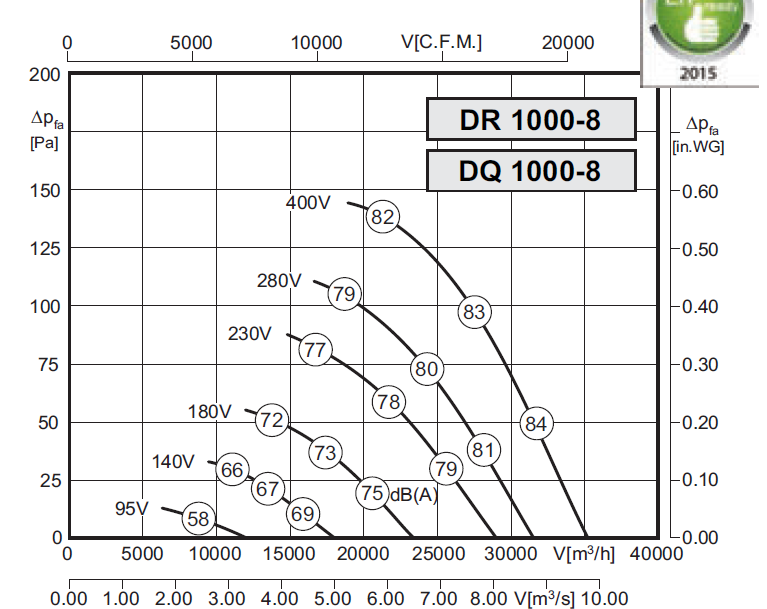
\includegraphics[scale=0.5]{editaveis/figuras/grafico_pressao_fluxo_ar}
	  \caption[grafico de pressão, fluxo de ar e tensão]{grafico de pressão, fluxo de ar e tensão\footnotemark}
	  \label{grafico_pressao_fluxo_ar}
	\end{figure}
	\FloatBarrier
	\footnotetext{Disponível em: http://www.axair-fans.co.uk/assets/product-resources/download/Axair\%20Fans\%20-\%20Rosenberg\%20Selection\%202013.pdf}
	\subsubsection{Torre de sustentação}
		  A torre de sustentação da turbina tem como função suportar todo o peso do rotor e da nacele e erguer este conjunto a uma altura onde as pás possam girar com segurança e distantes do solo. A altura da torre tem uma relação direta com a capacidade de produção de energia, sendo que quanto mais alto a torre for, maior será essa produção devido ao maior fluxo de vento. Com os ventos constantes, o que determinará a quantidade de energia a ser gerada é o diâmetro do rotor. O diâmetro do rotor da turbina tratada neste projeto é de 18,5 m, possuindo um torque médio em seu eixo de   4775, 5 N.m e com a necessidade de gerar 50 kW. A seguir uma breve relação entre o diâmetro do motor e a geração máxima de energia capaz de ser produzida por uma turbina eólica tradicional. \footnotemark
  \footnotetext{<http://www.fiec.org.br/artigos/energia/energia\_eolica.htm>. Acesso em 26 maio de 2015.}
  
  \begin{figure}[!h]
    \centering
    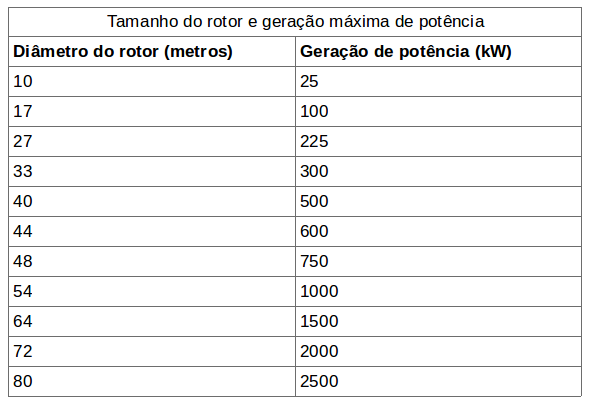
\includegraphics[scale = 0.5]{editaveis/figuras/tamanho_rotor}
    \label{tamanho_rotor}
    \caption[Tamanho do rotor e geração máxima de potência]{Tamanho do rotor e geração máxima de potência. \footnotemark}
   \end{figure}
   \FloatBarrier
   \footnotetext{Fonte: Associação Dinamarquesa da Indústria Eólica, Associação Americana de Energia Eólica.}
   
   Existem três tipos de torre utilizadas para a afinidade buscada: a tubular em aço, a tubular em concreto e a treliçada e quanto ao porte: pequeno, intermediário e grande porte. A turbina do projeto foi enquadrada como porte intermediário (10 - 250kW).  Devido ao aumento do peso dos componentes suportados pela nacele e das próprias pás ao longo dos anos, tem-se usado atualmente as torres tubulares de metais ou de concreto para assegurar a sustentação e suportar tensões provocadas por altitudes cada vez mais altas \footnotemark. Por este motivo e pela elevada preferência pelo mercado nesse tipo de torre, foi escolhido a torre tubular.
   \footnotetext{Disponível em: <http://www.cresesb.cepel.br/download/tutorial/tutorial\_eolica\_2008\_e-book.pdf>. Acesso em: 26 mai. 2015.}
   
   As torres cônicas tubulares podem ser compostos por aço, material relativamente barato e de montagem rápida podendo ser realizada no próprio lugar de instalação; Betão, que pode ser tanto construída no local como pré-moldado, porém é menos flexível que as torres de aço, ou podem ser híbridas, onde sua base é construída de concreto  e seu corpo principal de aço (As torres são frequentemente acoplada com parafusos às concretas bases sobre as quais repousam). \footnotemark
   \footnotetext{Fonte: Energias Renováveis: Energia Eólica 26/06/2014 Por : Luís Timóteo 3.}
   
   Depois de semanas de pesquisas, cruze de dados e comparações entre diversos modelos de torre, a equipe da frente de mecânica optou por utilizar uma torre de aço Q415 que passa por um processo de galvanização quente e pintado com spray, dando a capacidade de proteger a torre contra corrosão e ferrugem. \footnotemark
   \footnotetext{Disponível em: <http://www.chinahummer.cn/index.php/index/content/45>. Acesso em: 19 mai. 2015.}
   
   Partindo do princípio que a velocidade do vento necessária para a produção de energia desejada é a mínima do local de instalação das turbinas, definimos a altura como uma distância segura do solo apenas, tendo em vista que não precisamos colocar o rotor a uma determina altitude para que alcance uma determinada velocidade do vento. Desta forma, escolhemos uma torre com as seguintes especificações: 
   
   \begin{figure}[!h]
    \centering
    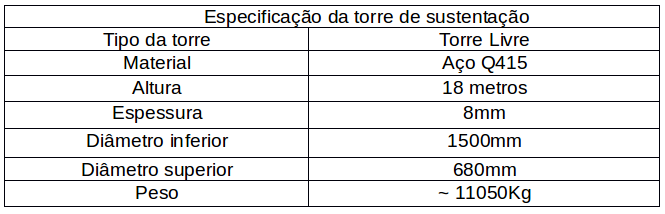
\includegraphics[scale = 0.5]{editaveis/figuras/torre_spec}
    \label{torre_spec}
    \caption[Especificação da torre de sustentação]{Especificação da torre de sustentação. \footnotemark}
   \end{figure}
   \FloatBarrier
   \footnotetext{Disponível em :< http://1047121.en.makepolo.com/products/50KW-Wind-Turbine-Generator-p41716180.html>. Acesso em 20 mai. 2015.}
   
   Quanto ao material utilizado nessa torre, trata-se de um Aço Inox 415. O aço inoxidável pertence à classe Martensítica e possui uma adição de elementos em sua composição química que aumenta a resistência à corrosão em relação aos martensíticos tradicionais. Comparado com os aços 410 e 420, o aço 415 contém uma quantidade menor de carbono, o que confere um diferencial para esta liga. Esta liga passa por um processo de têmpera para  que suas propriedades mecânicas e de dureza se elevem, posteriormente passando também por um processo de revenimento para aliviar as tensões internas do material provocadas pela têmpera. Sua aplicação é importante em ambientes onde o material está exposto a atrito, corrosão e abrasão, devido a estes fatores, a aplicação desta liga na construção de torres de sustentação para turbinas eólicas são constantes.\footnotemark
   \footnotetext{Disponível em:< http://www.megaligas.com.br/produtos\_aco\_inox\_S41500.asp>. Acesso em: 20 mai. 2015.}
   
	\subsubsection{Especificação do material usado na nacele}
		A Nacele é o compartimento situado no alto da torre e que comporta todos os componentes para a geração de energia responsável pela transformação de energia mecânica em energia elétrica. Seu tamanho e formato depende da presença de componentes e sua disposição em seu interior\cite{custodio2013}.Além dos componentes transformadores de energia, a nacele do projeto abrigará, também, todos os componentes envolvidos na obtenção da água pela umidade do ar. O desenvolvimento de materiais a serem utilizados devem ser destacados, uma vez que está relacionado diretamente com a produção de energia e com a redução de custos. A construção de turbinas eólicas devem ser preparadas para suportar diversas situações meteorológicas, existindo a necessidade de implantação de materiais mais leves e resistentes em todos os componentes. 	
	  
	As fibras de vidro pertencem a uma importante posição no mercado de materiais devido ao seu baixo coeficiente de dilatação térmica, facilidade de processamento, baixo custo e altas propriedades mecânicas e retenção desta em altas temperaturas3 e por isso escolhido para se construir a nacele.
	
	\begin{figure}[!htbp]
	 \centering
	  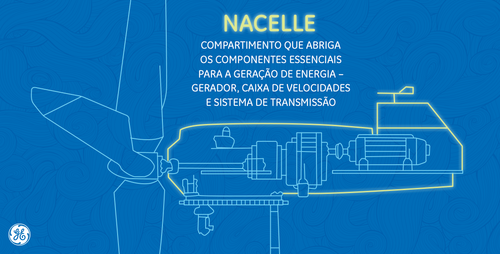
\includegraphics[scale=0.5]{editaveis/figuras/nacele}
	  \caption[nacele]{Nacele\footnotemark}
	  \label{nacele}
	\end{figure}
	\footnotetext{Disponível em: <http://www.tumblr.com/search/desenvolvemos\%20a\%20energia>}
	\subsubsection{Protótipos CATIA}
	  As peças necessárias para a construção da turbina foram prototipadas na ferramenta Catia \textregistered  e se encontram no 
	  anexo \ref{prototipos_catia}.
  
  \vfill
  \pagebreak
  \section{Matriz energética}
      
      Esta seção apresenta o funcionamento da matriz energética do sistema.
      
  	\subsection{Processo de produção de energia}
  		A transformação energética é fundamental ao projeto, é a partir dela que é proporcionado o funcionamento integral dos componentes da turbina afim de se captar a água do ar. Dentre as formas de energia utilizadas, a energia inicial é a contida nos ventos, fonte primária que alimentará todo o sistema. 

A força dos ventos ao entrar em contato com as pás do rotor, e devido a forma aerodinâmica das pás, faz com que haja rotação do mesmo. Para garantir a produção de energia, é necessário que os ventos possuam uma velocidade mínima suficiente para o funcionamento do sistema.  Ligado ao rotor, existe um eixo mecânico. Esse eixo mecânico é dividido em duas partes, uma de baixa velocidade e uma de alta velocidade. A função dos dois eixos é garantir um maior aproveitamento da energia de rotação do rotor transmitindo energia do eixo de baixa rotação para o eixo de alta rotação sendo estes interligados através da caixa multiplicadora. A função da caixa multiplicadora é multiplicar a rotação angular em relação ao eixo de baixa rotação e ao de alta rotação, atingindo assim nível necessário de rotação no gerador. Essa rotação das pás gira o eixo mecânico, que por sua vez está ligado ao gerador elétrico. Deste modo, temos a conversão da energia cinética dos ventos em energia mecânica de rotação através do eixo do rotor. Por fim, o gerador  converte a energia mecânica de rotação proveniente do eixo mecânico em energia elétrica. 

Para o rotor, considera-se o número de pás, desempenho aerodinâmico, materiais e o controle da rotação afim de evitar danos ao equipamento. A caixa multiplicadora uni os dois eixos a partir de engrenagens com o intuito de aumentar a velocidade da rotação angular, devido ao fato da rotação das pás ser baixa e o gerador exigir rotações maiores. A energia produzida é do tipo corrente alternada, pelo fato do gerador elétrico ser do tipo de indução, assíncrono, composto de estator e rotor, trifásico, o que facilita a distribuição direta aos componentes da turbina eólica. A tensão e a frequência de saída são controladas por uma unidade de condicionamento de potência que é definida de acordo com a necessidade dos equipamentos presentes na turbina eólica.

No caso do armazenamento em baterias, uma conversão para corrente continua é necessária. Essa conversão é feita por um conversor presente na torre de controle onde estarão as baterias.  As baterias utilizadas no projeto serão do tipo baterias estacionárias moura clean 220Ah, resistentes a altas temperaturas e dispensam a necessidade de resfriamento do ambiente. De acordo com o fabricante, são baterias ecoeficientes e estão de acordo com a regulamentação do CONAMA, além de serem indicadas para o armazenamento de energia de fontes renováveis. As baterias serão dispostas em uma sala para o seu armazenamento e utilizadas somente em caso de emergência. 

A seguir é apresentado o diagrama esquemático do caminho energético:
  	\subsection{Demanda energética}
  		O sistema que realizará o processo de retirada da água da umidade do ar terá a sua demanda energética suprida pela energia eólica, que é transformada em energia útil da mesma maneira que em aerogeradores usados atualmente. Para se estimar a necessidade de energia para todo o processo, incluindo o monitoramento, deve-se levar em consideração o consumo elétrico de todos os componentes.

A partir da análise dos componentes do sistema, chegou-se à uma lista de dispositivos que consomem energia elétrica, são eles: compressor de refrigeração, sensores (velocidade do vento e parâmetros de qualidade da água), aparelhos eletrônicos (casa de máquinas) e trocador de calor.

Os dois compressores usados serão de 18kW de potência. O trocador de calor, formado por duas ventoinhas, funciona com uma potência de 5kW. Tendo em vista o consumo de energia elétrico por lâmpadas e por computadores, estimou-se por meio de um simulador online o consumo da casa de máquinas, que será de 36kW, o que gera um consumo para cada turbina de 7.2kW. O consumo dos sensores será entorno de 1kW. Somando o gasto de todos os dispositivos, o consumo é de 47.2 kW por turbina.
Tendo em vista a eficiência do gerador elétrico de 90\% e a potência demandada pelo sistema, já considerando um excedente necessário para armazenamento, tem-se o valor da potência a ser captada de 55kW. Conhecendo essas informações, calcula-se o diâmetro do rotor a partir da seguinte equação:

\FloatBarrier
\begin{figure}[!ht]
\centering
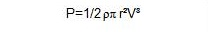
\includegraphics[scale=1]{figuras/eq_1energia}
\caption[Equação Rotor]{Equação diâmetro do rotor}
\label{rotor}
\end{figure}
\FloatBarrier

Onde P é a potência captada, $\rho$ é a massa específica do ar, r é o raio do rotor e V a velocidade do ar. Usando o valor da velocidade média dos ventos na região de 7m/s,m chegou-se ao valor do raio do rotor de 9,22m \cite{layton2011}.
A potência excedente produzida pelas 5 turbinas será de aproximadamente 40kW, já que a torre de controle usará energia da rede elétrica. A torre de controle só será abastecida pelas baterias em casos emergenciais, que serão utilizadas por até duas horas. Essa potência excedente será redirecionada para a rede por meio de um relé \cite{aldabo2002}.

  	\subsection{Dicionário de componentes}
  		\begin{itemize}
\item Pás do rotor: Capturam a energia existente no vento e a transfere para o cone do rotor; 
\item Cone do rotor: Liga as pás ao eixo de baixa velocidade da turbina eólica;
\item Eixo de baixa velocidade: Conecta o cone do rotor à caixa de engrenagens. 
\item Caixa de Multiplicadora: É utilizada para converter a baixa rotação em alta. A relação de engrenagens pode ser por exemplo de 1:40.
\item Eixo de alta velocidade: Ligado diretamente ao gerador elétrico. 
\item Gerador elétrico: Gerador de indução síncrono. 
\item Sistema de controle: Possui um microprocessador que monitora, continuamente, as condições do aerogerador e ativa o freio hidráulico, caso haja necessidade.
\end{itemize}
  	\subsection{Gerador Elétrico}
  		\FloatBarrier
\begin{figure}[!ht]
\centering
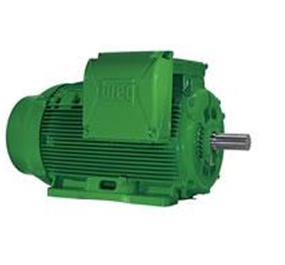
\includegraphics[scale=0.6]{editaveis/figuras/gerador}
\caption[Gerador]{Gerador\footnotemark}

\label{gerador}
\end{figure}
\footnotetext{Disponível em: http://ecatalog.weg.net/TEC\_CAT/tech\_motor\_dat\_web.asp}
\FloatBarrier

\textbf{Características do gerador}
\begin{longtable}{|p{4cm}|p{9cm}|}\hline
Carcaça	& 250S/M \\ \hline
Potência& 	75 kW\\ \hline
Frequência& 	60 Hz\\ \hline
Pólos	& 2\\ \hline
Rotação nominal	& 3565\\ \hline
Escorregamento	& 0,97\%\\ \hline
Tensão nominal	& 440 V\\ \hline
Corrente nominal& 	116 A\\ \hline
Corrente de partida& 	928 A\\ \hline
Ip / In	& 8,0\\ \hline
Corrente à vazio	& 33,5 A\\ \hline
Conjugado nominal& 	201 Nm\\ \hline
Conjugado de partida& 	290\%\\ \hline
Conjugado máximo	& 320\%\\ \hline
Categoria	& ---\\ \hline
Classe de isolação	& F\\ \hline
Elevação de Temperatura& 	80 K\\ \hline
Tempo de Rotor Bloqueado& 	20 s (quente)\\ \hline
Fator de serviço& 	1,25\\ \hline
Regime de serviço& 	S1\\ \hline
Temperatura Ambiente& 	$-20\,^{\circ}\mathrm{C}$ –+$-40\,^{\circ}\mathrm{C}$,
\\ \hline
Altitude	& 1000m\\ \hline
Proteção	& IPW55\\ \hline
Massa aproximada	& 535 kg\\ \hline
Momento de inércia	& 0,36268 kgm$^{2}$\\ \hline
Nível de Ruído	& 78 dB (A)\\ \hline
\caption[Gerador]{Gerador\footnotemark}
\end{longtable}

\footnotetext{Disponível em: http://ecatalog.weg.net/TEC\_CAT/tech\_motor\_dat\_web.asp}
\FloatBarrier
  	\subsection{Bateria}
  		O Banco de Baterias tem a função de armazenar a energia remanescente produzida pela turbina, com o intuito de manter todos os sensores e equipamentos da torre de controle, em caso de emergência, em perfeito funcionamento. Também será necessário uma bateria na turbina para manter o funcionamento dos sensores lá localizados.
O conjunto de baterias deve suprir toda a demanda da casa de máquinas. O consumo da casa de máquinas foi estimado em 36kW e dos sensores em torno de 1kW. Em caso de emergência, o Banco de Baterias deve manter o funcionamento da casa de máquinas por, aproximadamente, 2 horas.
 Para dimensionar o banco de baterias é necessário ter a potência dos equipamentos que serão alimentados pelas baterias, o tempo de funcionamento dos equipamentos e o uso do sistema. 
As baterias escolhidas foram as Baterias Estacionárias Moura Clean 220 Ah. As especificações estão em negrito no quadro a seguir:
\FloatBarrier
\begin{figure}[!ht]
\centering
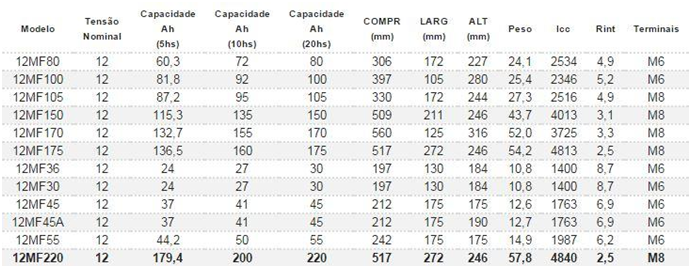
\includegraphics[scale=0.7]{editaveis/figuras/bateria}
\caption[Especificações das baterias]{Especificações das baterias\footnotemark}

\label{bateria}
\end{figure}
\footnotetext{Disponível em: https://www.energiapura.com/content/bateria-estacionária-moura-clean-220-ah}
\FloatBarrier

A potência e o tempo de funcionamento são utilizados para calcular o consumo. O consumo é calculado através da seguinte fórmula:
\FloatBarrier
\begin{figure}[!ht]
\centering
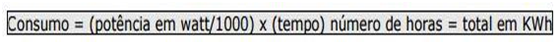
\includegraphics[scale=1]{editaveis/figuras/consumo}
\caption[Consumo]{Equação de consumo\footnotemark}
\label{consumo}
\end{figure}
\footnotetext{Disponível em: http://www.aneel.gov.br/arquivos/PDF/17-05\_materia1\_3.pdf}
\FloatBarrier

Substituindo os valores na fórmula, obtêm-se:
\FloatBarrier
\begin{figure}[!ht]
\centering
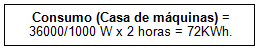
\includegraphics[scale=1]{editaveis/figuras/consumo_sub}
\caption[Consumo]{Cálculo do consumo da casa de máquinas}
\label{consumo}
\end{figure}
\FloatBarrier

Para mensurar a quantidade de baterias necessária, deve-se converter Kwh para Ah (ampère-hora). Para isso, utiliza-se a seguinte fórmula:
\FloatBarrier
\begin{figure}[!ht]
\centering
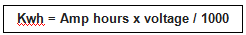
\includegraphics[scale=1]{editaveis/figuras/bateria_necessaria}
\caption[Equacao conversão]{Equação conversão Kwh para Ah\footnotemark}
\label{conversao}
\end{figure}
\footnotetext{Disponível em: http://www.hupsolar.com/questions-about-HUP-solar-batteries/How-to-convert-from-Kilowatt-hours-to-Amp-hours}
\FloatBarrier

Substituindo os valores na fórmula, obtêm-se:
\FloatBarrier
\begin{figure}[!ht]
\centering
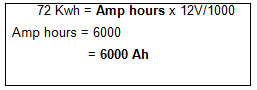
\includegraphics[scale=1]{editaveis/figuras/conversao_sub}
\caption[Conversao]{Cálculo da quantidade de baterias necessárias}
\label{conversao}
\end{figure}
\FloatBarrier

Analisando as especificações da bateria, observa-se a capacidade em Ah (5 horas) no valor de 179,4. Para o nosso projeto, considerando 2,5 horas, o valor é de aproximadamente 160 Ah. Isso significa que, para uma descarga de 2,5 horas serão consumidas 160 Ah.  

Para suprir a necessidade de manter a torre de controle ativa por duas horas, considerando que as baterias não possam ser descarregadas completamente e que tenha uma margem de segurança, deve-se utilizar várias baterias conectadas em série.
Dividindo a quantidade de ampères necessárias pela quantidade de ampères de uma bateria, é possível obter a quantidade de baterias necessárias para o projeto. O valor obtido é de 37 baterias.
Para manter os sensores que são acoplados na turbina em funcionamento em caso de emergência, a energia necessária é de aproximadamente 1 kW. Utilizando as fórmulas citadas acima; para manter o sistema de sensores por duas horas é necessário 2kWh.

Convertendo 2kWh, obtêm-se 166,66 Ah. Analisando a capacidade da bateria (aproximadamente 160 Ah (2,5 horas)), percebe-se que apenas uma bateria será o suficiente para suprir a necessidade dos sensores em caso de emergência (considerando a necessidade de aproximadamente 2 horas de funcionamento).

\FloatBarrier
\begin{figure}[!ht]
\centering
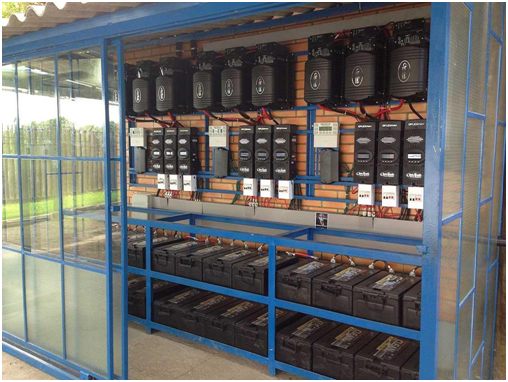
\includegraphics[scale=0.6]{editaveis/figuras/banco_bateria}
\caption[Banco baterias]{Banco de baterias MC 220 Ah na LACTEC em Curitiba\footnotemark}
\label{banco_bateria}
\end{figure}
\footnotetext{Disponível em: https://www.energiapura.com/content/bateria-estacion\%C3\%A1ria-moura-clean-220-ah}
\FloatBarrier

Terminada a fase de alimentação da própria turbina, a energia remanescente na ordem de KW é direcionada por cabeamento subterrâneo até a torre de controle. No meio do caminho, turbina eólica/torre de controle, será instalado um relé com a intenção de controlar a distribuição entre a rede elétrica da região através de um conversor eletrônico e a torre de controle. Em operação normal, a energia será direcionada preferencialmente para a rede elétrica local, evitando desperdícios e visando descontos no consumo energético da torre de controle. No caso de um eventual problema na distribuição energética local, a energia proveniente da turbina será direcionada diretamente para a torre de controle, suprindo suas necessidades de operação e o excedente é direcionada ao carregamento das baterias. A energia na casa de máquinas será utilizada para alimentar computadores, iluminação, tratamento UV e convertida para a alimentação das baterias. 

Para gerarmos energia temos pás, rotor, transmissão por eixo mecânico e gerador elétrico. A partir da energia produzida, os demais componentes da turbina são alimentados eletricamente. Os componentes que recebem alimentação elétrica proveniente do gerador  diretamente na turbina são:
\begin{itemize}
\item Compressor;
\item Sensores;
\item Ventoinha de Ingestão de Ar;
\item Ventoinha de Exaustão de Ar;
\item Sistema de Frenagem.
\end{itemize}

Depois disso, toda a energia remanescente é direcionada para a rede elétrica local/torre de controle. Na central temos os demais componentes que consumirão parte dessa energia. Alguns dos componentes são:
\begin{itemize}
\item Lâmpadas de iluminação;
\item Computadores;
\item Sistema de tratamento;
\item Conversor de Corrente;
\item Baterias.

\end{itemize}

A seguir é apresentado o diagrama esquemático do caminho energético:
  
  \vfill
  \pagebreak
  \section{Sistema de monitoramento e controle da qualidade da água}
      
      Optou-se por sensores os quais não são integrados em um sistema próprio isolado que já disponibiliza a leitura das grandezas
      referentes às propriedades analisadas: turbidez, oxigênio dissolvido, etc. Tal escolha foi feita visando agrupar todas as
      leituras em uma só interface controlada por um microcontrolador capaz de processar os sinais de saída de todos os sensores.
      Além disso, percebeu-se que fazendo esse tipo de abordagem (preferência por sensores não integrados à um sistema isolado)
      é possível baratear o projeto, uma vez que os sensores integrados são bem mais caros.
    
    \subsection{Monitoramento do sistema de captação}
      
      Esta seção apresenta os sensores que serão utilizados para o monitoramento do sistema de captação
      de água, que compreende as turbinas e suas respectivas estruturas.
      
      \subsubsection{Anemômetro Ultrassônico}
  
  Para compor o sistema de monitoramento das turbinas e a avaliação da produção de energia, sentiu-se a necessidade de utilizar
  o anemômetro. O anemômetro é um sensor que possibilita medir a velocidade e a direção em que o ar se desloca. Há vários tipos
  de anemômetros no mercado, com diferentes métodos de medição, precisão e manutenção. Entre os anemômetros comerciais, o tipo
  ultrassónico é o que possui maior precisão, confiabilidade nos valores medidos em qualquer tipo de ambiente, rápida resposta
  e maior tempo de manutenção em comparação aos outros tipos no mercado.
  
  O anemômetro ultrassônico possibilita a medição da velocidade do vento , por meio da velocidade do som no ar. Possui usualmente
  sensores ultrassônicos dispostos em formato de tetraedro, com um sensor piezolétrico em cada extremidade \cite{ribeiro06}.
  Primeiramente para inicializar o processo de medição, o anemômetro produz um sinal de referência, que é enviado ao 
  transdutor-transmissor, logo depois que este recebe o sinal, emite-se um sinal ultrassônico, que no decorrer do caminho até 
  chegar ao transdutor-receptor, sofre interferências da velocidade causadas pelo deslocamento do vento. Quando o sinal finalmente
  chega ao transdutor receptor o sinal é processado e há a alteração do sinal de referência que é quantificado \cite{pereira07}.
  
  Dentre os modelos disponíveis no mercado escolheu-se o anemômetro ultrassônico Young Modelo 86000.
  Este modelo além de ser compacto, possui baixo consumo, marcação CE e um bom custo-benefício.
  
  O modelo 86000 custa em torno de \$1390,00 com os impostos sobre seu preço integral e de frete, seu custo em reais
  é em torno de R\$ 7.579,50.
  
  \begin{figure}[!htbp]
    \centering
    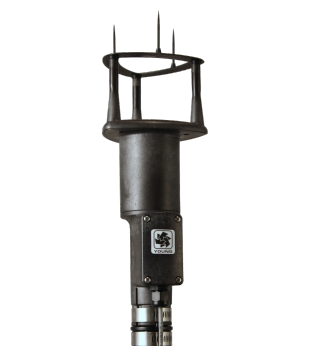
\includegraphics[scale=0.5]{editaveis/figuras/anemometro}
    \caption[Anemômetro ultrassônico Modelo 86000]
    {Figura ilustrativas do Anemômetro ultrassônico Modelo 86000 \footnotemark .}
    \label{anemometro}
  \end{figure}
  \footnotetext{Fonte: R.M. YOUNG COMPANY - OPERATING INSTRUCTIONS Model 86000 Ultrasonic Anemometer.}
  
  Abaixo as especificações técnicas do modelo 86000:
  
  \begin{figure}[!htbp]
    \centering
    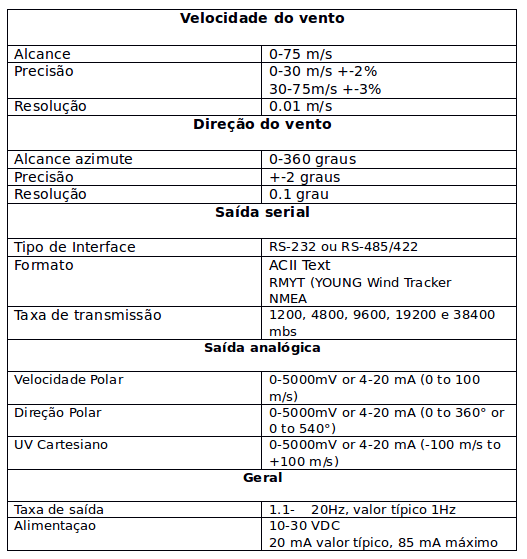
\includegraphics[scale=0.5]{editaveis/figuras/anemometro_spec}
    \caption[Especificações técnicas do anemômetro Modelo 86000]
    {Especificações técnicas do anemômetro Modelo 86000 \footnotemark .}
    \label{anemometro_spec}
  \end{figure}
  \footnotetext{Fonte: R.M. YOUNG COMPANY - OPERATING INSTRUCTIONS Model 86000 Ultrasonic Anemometer.}
  
  
  
           
      \subsubsection{Sensor de rotação (Efeito Hall)}
	
	O sensor escolhido foi o US1881 \textit{Hall Latch} – \textit{High Sensitivity} da Melexis
	(\textit{Microeletonic Integrated Systems}), que é um sensor
	digital disponível na loja virtual SparkFun a U\$ 0,95 (este valor não considera as taxas de envio). Devido à sua larga
	faixa de operação de tensão (VDD) e temperatura, esse sensor é adequado para a aplicação proposta \cite{melexis}.
	
	O sensor detecta a presença de polos magnéticos. Existem dois tipos de encapsulamentos, cujas lógicas de funcionamento
	são inversas e são apresentadas a seguir:
	
	\begin{figure}[!htbp]
	  \centering
	  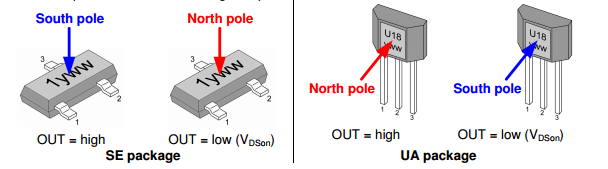
\includegraphics[scale=0.4]{editaveis/figuras/encapsulamento_sensor_efeito_hall}
	  \caption[Tipos de encapsulamento do sensor de efeito Hall]{Tipos de encapsulamento do sensor de efeito Hall \cite{melexis}.}
	  \label{encapsulamento_sensor_efeito_hall}
	\end{figure}
	
	\begin{figure}[!htbp]
	  \centering
	  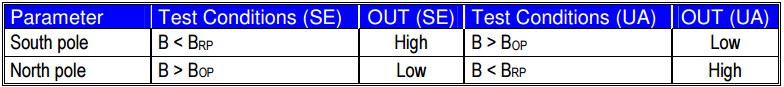
\includegraphics[scale=0.5]{editaveis/figuras/funcionamento_sensores_encapsulamento}
	  \caption[Lógica de funcionamento dos sensores considerado os encapsulamentos]
	  {Lógica de funcionamento dos sensores considerado os encapsulamentos (T = $-40^\circ\mathrm{C}$ a $150^\circ\mathrm{C}$, VDD = 3,5V a 24V) \cite{melexis}.}
	  \label{funcionamento_sensores_encapsulamento}
	\end{figure}
	
	Onde:
	
	\begin{itemize}
	 \item $B_{op}$ = Densidade de fluxo magnético aplicado no lado que tem a marca do encapsulamento que liga o condutor de saída.
	 \item $B_{rp}$ = Densidade de fluxo magnético aplicado no lado que tem a marca do encapsulamento que desliga o condutor de saída.
	\end{itemize}
	
	Abaixo é apresentada uma tabela com a os valores máximos suportados de diversos parâmetros 
	(informações necessárias para a estimação de consumo energético do sistema):
	
	\begin{figure}[!htbp]
	  \centering
	  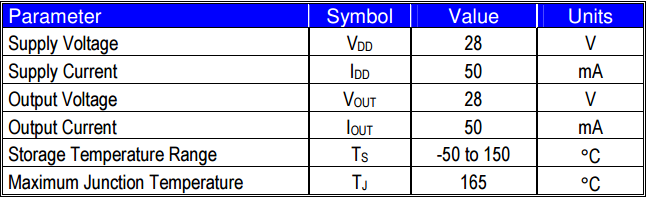
\includegraphics[scale=0.5]{editaveis/figuras/sensor_rotacao_max_valores}
	  \caption[Máximos valores suportados pelo sensor de rotação.]
	  {Máximos valores suportados pelo sensor de rotação \cite{melexis}.}
	  \label{sensor_rotacao_max_valores}
	\end{figure}
	
	Deve-se adquirir o sensor o qual tem o sufixo $\mathrm{L}$, uma vez que esse é o tipo que suporta a maior variação de
	temperatura: $-40^\circ\mathrm{C}$ a $150^\circ\mathrm{C}$ \cite{melexis}.
	
	As tabelas com as descrições/especificações do sensor são apresentadas abaixo:
	
	\begin{figure}[!htbp]
	  \centering
	  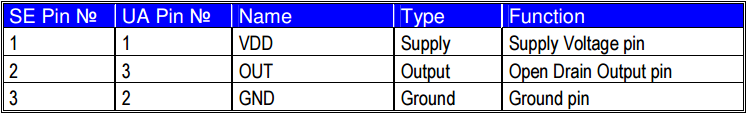
\includegraphics[scale=0.5]{editaveis/figuras/sensor_rotacao_pinagem}
	  \caption[Pinagem e função dos pinos do sensor de rotação]
	  {Pinagem e função dos pinos do sensor de rotação \cite{melexis}.}
	  \label{sensor_rotacao_pinagem}
	\end{figure}
	
	\begin{figure}[!htbp]
	  \centering
	  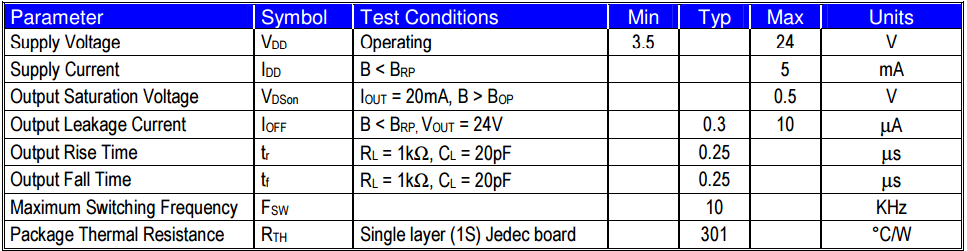
\includegraphics[scale=0.4]{editaveis/figuras/sensor_rotacao_spec_eletrica}
	  \caption[Pinagem e função dos pinos do sensor de rotação]
	  {Pinagem e função dos pinos do sensor de rotação \cite{melexis}.}
	  \label{sensor_rotacao_spec_eletrica}
	\end{figure}
	
	\begin{figure}[!htbp]
	  \centering
	  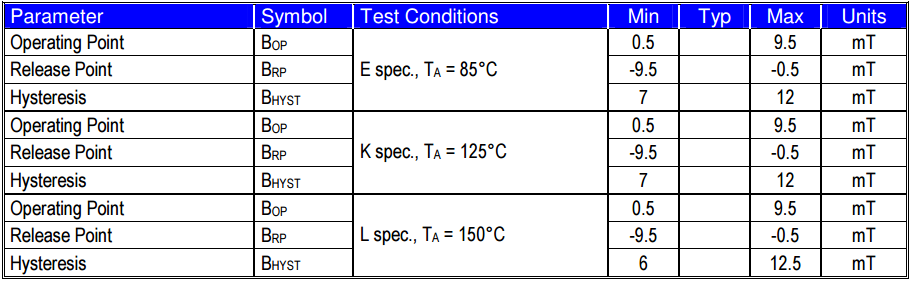
\includegraphics[scale=0.5]{editaveis/figuras/sensor_rotacao_spec_mag}
	  \caption[Especificações elétricas do sensor de rotação]
	  {Especificações elétricas do sensor de rotação \cite{melexis}.}
	  \label{sensor_rotacao_spec_mag}
	\end{figure}
	
	As figuras ~\ref{sensor_rotacao_idd_vs_vdd} e ~\ref{sensor_rotacao_vdd_vs_temperatura} apresentam dois gráficos
	de performance do sensor.
	
	\begin{figure}[!htbp]
	  \centering
	  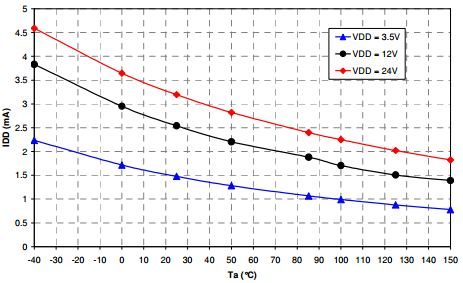
\includegraphics[scale=0.5]{editaveis/figuras/sensor_rotacao_idd_vs_vdd}
	  \caption[Sensor de rotação -  IDD vs VDD]
	  {Sensor de rotação -  IDD vs VDD \cite{melexis}.}
	  \label{sensor_rotacao_idd_vs_vdd}
	\end{figure}
	
	\begin{figure}[!htbp]
	  \centering
	  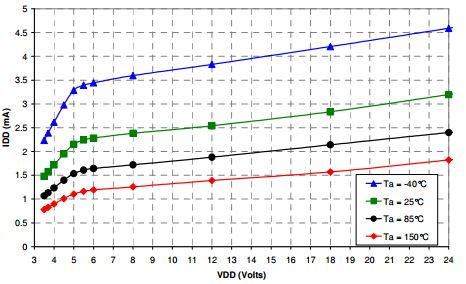
\includegraphics[scale=0.5]{editaveis/figuras/sensor_rotacao_vdd_vs_temperatura}
	  \caption[Sensor de rotação -  VDD vs Temperatura]
	  {Sensor de rotação -  VDD vs Temperatura \cite{melexis}.}
	  \label{sensor_rotacao_vdd_vs_temperatura}
	\end{figure}
	
	Para medir a velocidade de rotação da turbina, pretende-se elaborar uma montagem como a mostrada a seguir:
	 
	\begin{figure}[!htbp]
	  \centering
	  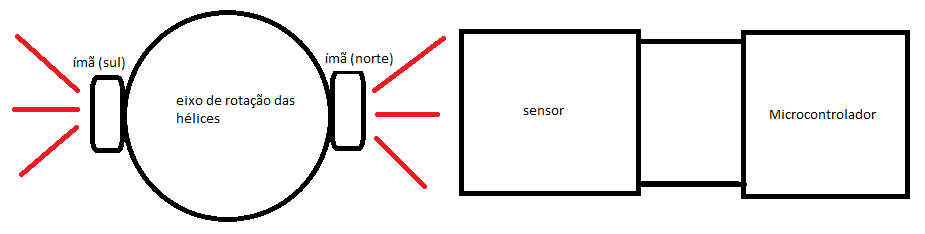
\includegraphics[scale=0.4]{editaveis/figuras/sensor_rotacao_monitoramento_velocidade}
	  \caption[Esquema simplificado de funcionamento do monitoramento da velocidade do eixo]
	  {Esquema simplificado de funcionamento do monitoramento da velocidade do eixo.}
	  \label{sensor_rotacao_monitoramento_velocidade}
	\end{figure}
	
	Uma vez que o sinal é digital, não há necessidade de filtragem do sinal, basta aplicar uma tensão VDD que seja suportada
	pelo microcontrolador (5V por exemplo).
	
	\begin{figure}[!htbp]
	  \centering
	  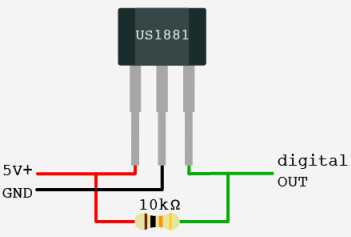
\includegraphics[scale=0.4]{editaveis/figuras/sensor_rotacao_conexao}
	  \caption[Esquema de conexão do sensor de rotação]
	  {Esquema de conexão do sensor de rotação. \footnotemark}
	  \label{sensor_rotacao_conexao}
	\end{figure}
	\footnotetext{Disponível em: <http://bildr.org/2011/04/various-hall-effect-sensors/>.}
	
	O algoritmo para determinar a velocidade de rotação das hélices deve, portanto, avaliar a frequência em que a saída do
	sensor apresenta-se em nível lógico alto (borda de subida) ou baixo (borda de descida) e com base nisso, efetuar o
	cálculo da velocidade (rpm, por exemplo).
      \subsubsection{Acelerômetro piezoelétrico}

  As pás da turbina quando realizam rotações, criam vibrações no local onde elas estão girando. Como todas as outras partes
  estão interligadas, isso gera uma vibração em toda a estrutura. Essas vibrações são forças de variadas intensidades sendo
  geradas em vários pontos. Como qualquer estrutura mecânica, há um limite para as forças internas e externas agindo no sistema
  para que este não entre em colapso. A fim de se ter um controle maior sobre as vibrações causadas na estrutura para que
  estes eventos não causem sérios danos à turbina e seus componentes, serão utilizados acelerômetros como indicadores da
  vibração com o propósito de se monitorar os possíveis danos à estrutura.
  
  Os acelerômetros piezoelétricos (sensores de vibração) são componentes sensíveis a aplicações de forças neles. Funcionam da
  seguinte forma: as forças que são aplicadas a ele faz com que este se deforme, assim, produz cargas elétricas que são
  proporcionais às forças recebidas. Como a carga é proporcional à força e a massa é uma constante, a carga também é proporcional
  à aceleração. Dessa forma, estes componentes conseguem medir vibrações/acelerações (movimentação) de objetos relacionando com
  a proporção entre as forças aplicadas e as cargas elétricas produzidas \footnotemark.
  \footnotetext{Fonte: <https://br.omega.com/prodinfo/acelerometros.html>.}
  
  Foram feitas várias pesquisas a cerca de qual o melhor acelerômetro ser usado para o projeto, levando em conta preço, tipo do
  sensor, sensibilidade (mV/g). Dentre os encontrados, muitos estavam fora da faixa de sensibilidade adequada para o porte do
  projeto. Nos sites pololu.com \footnotemark \footnotetext{<https://www.pololu.com>} e
  sparkfun.com \footnotemark \footnotetext{<https://www.sparkfun.com>} não se encontrou acelerômetros piezoelétricos adequados, pois suas faixas
  de sensibilidade estão geralmente entre 3 g, 6 g, 12 g. Vale lembrar que 1 g = 9,8 $m/s^2$ (aceleração da gravidade). O sensor 
  escolhido foi decidido pela compatibilidade com a alta tolerância de impactos que ele resiste. Entretanto, no endereço 
  eletrônico \footnotemark \footnotetext{<https://www.imi-sensors.com/Products.aspx?m=339A30>} onde foi encontrado, o revendedor colocou o preço de \$ 0,00. A seguir se encontra uma imagem do
  sensor e logo após todas as especificações deste:
  
  \begin{figure}[!htbp]
    \centering
    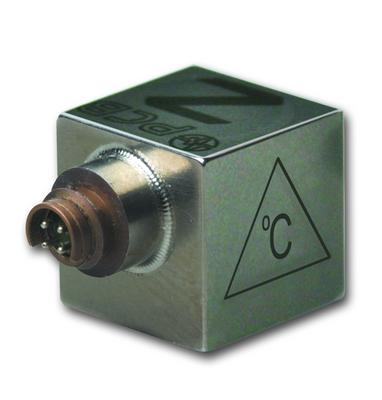
\includegraphics[scale=0.5]{editaveis/figuras/acelerometro}
    \caption[Acelerômetro para vibrações (\textit{Triaxial ICP accelerometer})]
    {Acelerômetro para vibrações (\textit{Triaxial ICP accelerometer}).}
    \label{acelerometro}
  \end{figure}
  
  A figura ~\ref{desempenho_acelerometro} ilustra o desempenho do acelerômetro. A figura ~\ref{param_eletrico_acelerometro} traz
   os parâmetros elétricos do acelerômetro. A figura ~\ref{ambiente_acelerometro} mostra os dados relativos ao ambiente.
  
  \begin{figure}[!htbp]
    \centering
    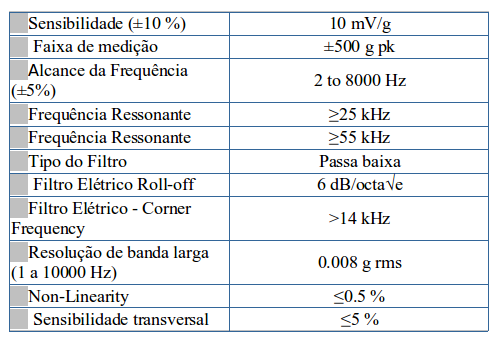
\includegraphics[scale=0.5]{editaveis/figuras/desempenho_acelerometro}
    \caption[Desempenho do acelerômetro]
    {Desempenho do acelerômetro.}
    \label{desempenho_acelerometro}
  \end{figure}
   
    \begin{figure}[!htbp]
	\centering
	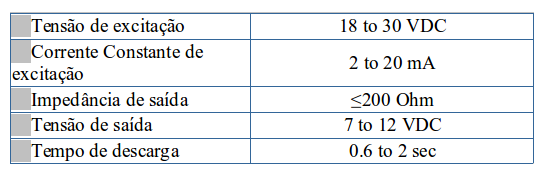
\includegraphics[scale=0.5]{editaveis/figuras/param_eletrico_acelerometro}
	\caption[Parâmetros elétricos do acelerômetro]{Parâmetros elétricos do acelerômetro.}
	\label{param_eletrico_acelerometro}
      \end{figure}
   
    \begin{figure}[!htbp]
      \centering
      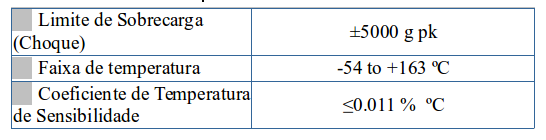
\includegraphics[scale=0.5]{editaveis/figuras/ambiente_acelerometro}
      \caption{Relativo ao ambiente.}
      \label{ambiente_acelerometro}
    \end{figure}
      
    \subsection{Monitoramento da qualidade da água}
    
      \subsubsection{Sensor de pH}
O sensor de pH da água é de extrema importância para o projeto  pois monitora um dos índices de qualidade da água especificados pela ANA(agência nacional de águas). 

Para aplicações industriais, o método de medição de pH mais empregado é o eletrodo de vidro. Os eletrodos de pH possuem basicamente o mesmo funcionamento que as baterias: transferem uma tensão mínima que poderá ser detectada por um medidor ou um regulador de pH. A diferença é que os eletrodos de pH não produzem tensão de forma contínua, a não ser quando são introduzidos num líquido. Os sensores foram pesquisados principalmente nos sites \footnotemark \footnotetext{https://www.sparkfun.com}, \footnotemark \footnotetext{https://www.pololu.com} e \footnotemark \footnotetext{http://www.vernier.com}, o sensor a ser utilizado no projeto pode ser visto na imagem abaixo. 
	\begin{figure}[!htbp]
	  \centering
	  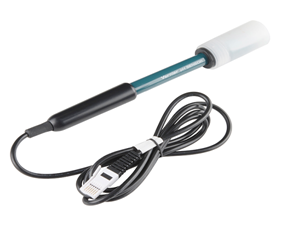
\includegraphics[scale=1]{editaveis/figuras/sensor_ph}
	  \caption[Sensor de pH]{Sensor de pH}
	  \label{sensor_ph}
	\end{figure}
	\FloatBarrier
Um ponto importante sobre os sensores de pH é o fato deles apresentarem erros de medição quando colocados em água destilada. Por este motivo, para se obter uma maior precisão na medição dos sensores, deve-se colocar o sensor de pH no tanque de água já adicionada de sais. Um dos fatores importantes para a escolha do Vernier sensor é o fato deste dispositivo ser compatível com softwares já existentes, além do fato dele possuir calibração via software, o que irá facilitar o manuseio do mesmo.

	A escolha do tipo de sensor de pH a ser utilizado depende também da temperatura do líquido a ser aferido. A faixa de temperatura do sensor escolhido é adequada para a aplicação, já que o sensor possui uma faixa de atuação de 5 a $80\,^{\circ}\mathrm{C}$. Como o sensor de pH funciona por meio de comparação, deve ser preparada uma solução para ser adicionada ao sensor. Recomenda-se a utilização de soluções de pH 4, 7 ou 10. A seguir, podem ser observadas as receitas das soluções de pH que podem ser utilizadas.

\begin{table}[h]
\centering 
\begin{tabular}{|c|p{12cm}|}\hline
pH 4,0 	& Adicionar 2.0 mL de 0.1 MHCl para cada 1000 mL de 0.1 M Hidrogenoftalato de potássio.\\\hline
pH 7,0 	& Adicionar 582 mL de 0.1 MNaOH para cada 1000 mL de 0.1 M di-hidrogenofosfato de potássio.\\\hline
pH 10,0 & 	Adicionar 214 mL de 0.1 MNaOH para 1000 mL de 0.05 M bicarbonato de sódio.\\ \hline
\end{tabular}

\caption{Preparo da solução para o sensor de pH}
\end{table}
\FloatBarrier

\begin{center}\textbf{Especificações técnicas do sensor de pH}
\end{center}

\begin{table}[h]
\centering 
\begin{tabular}{|c|p{9cm}|}\hline
Faixa de temperatura&5- $80\,^{\circ}\mathrm{C}$\\ \hline
Tensão de saída	&0.25 volts/pH\\ \hline
Faixa de atuação(pH)& pH 0-14\\ \hline
Preço&R\$ 78,95\\ \hline
Acurácia&+/- 0.2 unidades de pH\\ \hline
Tempo de resposta&	90\% da leitura acontece em 1 segundo\\ \hline
Resolução&13 bits\\ \hline
\end{tabular}

\caption{Especificações técnicas do sensor de pH}
\end{table}
\FloatBarrier
      \subsubsection{Sensor de turbidez}

  A turbidez foi um dos parâmetros escolhidos para o monitoramento da qualidade da água. Resumidamente este parâmetro é definido como o grau de intensidade que um feixe de luz atravessa a água, quanto menor for essa intensidade, mais sólidos em suspensão estão presentes na amostra da água analisada, logo, menor será sua qualidade, segundo a CETESB.
  
  Para medir-se este parâmetro utilizará o sensor óptico de turbidez o turbidímetro nefelométrico, que utiliza detectores fotoelétricos para medir a intensidade da luz emitida pelo próprio sensor para indicar o grau de turbidez da amostra de água.
  
  Dentre os sensores disponíveis no mercado optou-se pelo produto da empresa Ponsel, o modelo a ser utilizado é o PONSEL DIGISENS Turbidity Sensor \footnotemark, os motivos por ter escolhido este produto é sua qualidade, robustez, certificação, custo-benefício, garantia e confiabilidade da empresa.
  \footnotetext{Disponível em: <http://www.fondriest.com/ponsel-digisens-turbidity-sensor.htm>}
  
  Por se tratar de um produto importado o preço para adquirir um sensor é de R\$ 4.822,99 com impostos e frete inclusos.
  
  \begin{figure}[!h]
    \centering
    \includegraphics[scale = 0.5]{editaveis/figuras/turbidez_spec}
    \label{fishbone}
    \caption[Especificações do sensor PONSEL DIGISENS Turbidity Sensor]
      {Especificações do sensor PONSEL DIGISENS Turbidity Sensor. \footnotemark}
  \end{figure}
  \FloatBarrier
  \footnotetext{Disponível em: <http://www.fondriest.com/ponsel-digisens-turbidity-sensor.htm>}
  
      \subsubsection{Sensor de nível da água}

  Sensores de nível medem o nível de substâncias que fluem, sejam estes produtos líquidos, pós ou sólidos granulares. Sua medição se dá em detecção de nível, em que existe um sinal que aponta se a substância está acima ou abaixo de um parâmetro, ou medição contínua, onde, dentro de uma faixa de operação, o nível exato é mensurado \cite{quintanilha13}.
  
  A escolha do sensor usado na aplicação depende de vários fatores, entre eles: estado físico do material (alguns sensores são mais adequados para medições de líquidos, enquanto outros têm a melhor aplicação na medição de sólidos granulares ou pós), sensores de temperatura, sendo aplicado em ambientes controláveis. 
  
  Os sensores de níveis que serão implementados nos reservatórios de água do projeto são os sensores do tipo boia magnética da marca Gems Sensores e Controls, eles foram escolhidos por serem confiáveis e baratos, custam em torno de R\$ 120.0, além do mais, sua melhor aplicação é na detecção de nível, pois não tem boa acurácia. Esses sensores também foram escolhidos pela fácil conexão com os microcontroladores e envio de dados. A importância desses sensores no projeto consiste em saber o nível da água para fazer o controle do fluxo da água, decidindo se continua o processo de fluxo ou então se cessa o processo de passagem da água pelo motivo do tanque já estar com sua capacidade máxima atingida. 

  Nesse tipo de sensor, a boia move de acordo com a superfície da água, indicando o nível. A medição pode ser quanto contínua, gerando um sinal analógico ao variar a resistência da haste que segura o flutuador, por exemplo; quanto discreta, simplesmente detectando um limiar, como em uma caixa d’água.
  
%   \begin{figure}[!h]
%     \centering
%     \includegraphics[scale = 0.5]{editaveis/figuras/sensor_nivel_boia}
%     \label{sensor_nivel_boia}
%     \caption{Sensor de nível tipo boia}
%    \end{figure}
%    \FloatBarrier
   
  Sensores do tipo boia magnético funcionam tanto na vertical quanto na horizontal, na horizontal o fechamento do contato ocorre com a aproximação de um campo magnético. Já um flutuador magnético vertical é comumente colocado no topo do tanque e a boia é instalada sob uma mola, que ao ser tencionado, resulta em um movimento vertical tanto do núcleo quanto da haste, levando o magneto para fora, retirando o contato com a chave. 
  
  \begin{figure}[!h]
    \centering
    \includegraphics[scale = 0.6]{editaveis/figuras/sensor_nivel_spec}
    \label{sensor_nivel_spec}
    \caption{Especificações do sensor de nível}
   \end{figure}
   \FloatBarrier
   
   \vfill
    
    \subsection{Controle dos dados monitorados}
    
      No projeto de captação de água a partir da umidade do ar o microcontrolador irá ser embarcado em algum ponto estratégico para que se possa controlar as funções ou ações do projeto. O microcontrolador que se utilizará tem a capacidade de integrar elementos adicionais em sua estrutura interna como memórias para registro e controle de dados e sensores de medição quando usados com condicionamento de sinais.
      
      \subsubsection{Placas de aquisição de dados}
      
	Placas de aquisição de dados são utilizadas para recolher informação do mundo real e gera dados que podem ser manipuladas pelo computador. Essas placas usam processamentos de sinais para obtenção das informações desejadas. Os sensores usados convertem os parâmetros medidos em sinais eletrônicos e são processados pelo microcontrolador. Os dados são analisados, monitorados e guardados em um computador. 
	
	A placa de aquisição de dados multifunções, série M, fabricante National Instruments apresenta funcionalidades otimizadas para as aplicações que o projeto demanda. Ela é ideal para o registro e controle de dados e para interface com sensores de medições e processamentos de sinais. A figura a seguir apresentam as especificações da placa.
	
	\begin{figure}[!ht]
	  \centering
	  \includegraphics[scale=0.6]{editaveis/figuras/placa_aquisicao_spec}
	  \caption[Especificações técnicas da placa de aquisição de dados utilizada]
	      {Especificações técnicas da placa de aquisição de dados utilizada. Fonte: \cite{national04}.}
	\label{placa_aquisicao_spec}
	\end{figure}
	
	A interface da placa com os sensores de medição é feita através de um bloco conector I/O CB – 68LP da mesma fabricante. Este conector ilustrado na imagem abaixo tem 68 terminais para uma ligação fácil com os sensores de medição.
    
	\begin{figure}[!ht]
	  \centering
	  \includegraphics[scale=0.5]{editaveis/figuras/bloco_conector_placa_aquisicao}
	  \caption[Bloco conector I/O CB-68LP]
	      {Bloco conector I/O CB-68LP. Fonte: \cite{national04}.}
	\label{bloco_conector_placa_aquisicao}
	\end{figure}
	
	As dimensões do bloco conector I/O CB – 68LP são de 14,35 cm por 10,74 cm. A ligação entre a placa de aquisição de dados e o bloco conector exige um cabo R6868 Ribbon I/O, que apresentam nas suas extremidades um conector de 68 terminais. 
	
	O custo para a utilização da placa de aquisição de dados com o bloco conector e o cabo de 68 terminais se totaliza em \$580,00.
	
    \pagebreak
    \subsection{Processo de adição de sais minerais}
    
      
A água potável em sua forma pura é conhecida como água destilada. Esta água é desprovida de sais minerais ou de gases.
O consumo constante de água destilada pode ser prejudicial aos seres humano devido ao fato de a ingestão diária de sais
minerais ser complementada pelos sais presentes na água mineral. Segundo resolução da Anvisa, toda água mineral no país 
que possua como objetivo ser comercializada deve ser adicionada de sais minerais. Visando seguir esta especificação e
visando não provocar um impacto na saúde dos habitantes de Acarí optou-se por adicionar sais minerais básicos à água
retirada da umidade do ar já que a falta de sais minerais na dieta dos habitantes pode levar a doenças para os mesmos,
tais como diarreia e desidratação.

Uma das propriedades mais importantes da água é o fato de ser uma substância polar, capaz de associar-se a outras substâncias 
polares ou iônicas para formar soluções aquosas. O processo de solubilização para a planta de abastecimento de água por meio
da umidade do ar pode ser realizado por um simples processo de mistura entre os sais contidos em um reservatório e a água
provinda da turbina. Portanto, será implementado um sistema de injeção e monitoramento de sais minerais à água provinda da
turbina que contará com processos mecânicos e digitais.

\subsubsection*{Quantidade e especificações dos sais minerais adicionados}

  Segundo a Anvisa, a água adicionada de sais  deve ser possuir pelo menos 30ml de um dos seguintes sais, de grau alimentício:
  bicarbonato de cálcio, bicarbonato de magnésio, bicarbonato de potássio, bicarbonato de sódio, carbonato de cálcio, carbonato
  de magnésio, carbonato de potássio, carbonato de sódio, cloreto de cálcio, cloreto de magnésio, cloreto de potássio, cloreto
  de sódio, sulfato de cálcio, sulfato de magnésio, sulfato de potássio, sulfato de sódio, citrato de cálcio, citrato de magnésio,
  citrato de potássio e citrato de sódio.
  
  \begin{table}[h]
    \centering
    \begin{tabular}{|c|c|}
    
    \hline
    Substância & Quantidade(mg)\\
    \hline                               
    Cálcio & 25\\
    \hline                               
    Magnésio & 6,5\\
    \hline                               
    Potássio & 50\\
    \hline                               
    Sódio & 60\\
    \hline
    \end{tabular}
    \caption{Quantidades limites de sais minerais para cada 100 mililitros de água \cite{anvisa05}.}
  \end{table}
  
\subsubsection{Mecanismos para a adição dos sais minerais}

  Para a adição de sais minerais na água, será implementado um mecanismo baseado em equipamentos já existentes, que injetarão
  sais minerais na água provinda da turbina. Para a realização de um processo automático de inserção de sais, será necessária 
  a utilização de um dosador automático, que varia a dosagem de uma substância de acordo com as concentrações da mesma na mistura 
  que será constantemente verificada. Existem equipamentos como o Dosimat 865, da empresa Metrohm, que possui o modo de operação
  CNT D: ao ser inserida a concentração final que se deseja de uma substância, o dosador é capaz de determinar o volume de água
  a ser adicionado para que a concentração desejada seja mantida.
  
\subsubsection{Funcionamento básico do sistema}

  \begin{itemize}
   
   \item O \textbf{sistema de controle} terá a função de enviar comandos e desta forma realizar o controle mecânico da comporta 
   que abre e fecha o tanque de armazenamento da água retirada da umidade do ar. Este sistema terá acesso direto ao aparelho
   dosador e ao sistema de sensoriamento, pois, por meio dele terá acesso às concentrações dos sais no tanque de adição. 
   Quando as concentrações de sais no tanque de adição estiverem altas, a comporta se abrirá e mais água será adicionada à 
   mistura. Por outro lado, quando as concentrações de sais estiverem baixas no tanque de adição, os comandos serão dados
   para que a comporta seja fechada. Este processo ocorrerá até que as concentrações ideais dos sais sejam atingidas.
   
   \item A \textbf{válvula de retenção} será utilizada para que a água flua apenas em um sentido, que no caso do esquemático 
   seria da esquerda para a direita. Isto impedirá que a água já adicionada de sais retorne ao tanque da água retirada da
   umidade do ar.
   
   \item O \textbf{tanque para adição de sais} será o reservatório que conterá a água adicionada de sais. Neste tanque, além
   de ocorrer a adição de sais, ocorrerá também o processo de mistura para que a solubilização dos sais na água aconteça de
   forma uniforme.
   
   \item Para o \textbf{sensoriamento} do tanque de adição de sais poderá ser utilizado um sensor de condutividade.
   Este sensor possui grande aplicabilidade a este sistema de sensoriamento, pois “A água tem um forte poder de dissociação,
   pode separar o material dissolvido em íons carregados eletronicamente. Como consequência, o material dissolvido aumenta
   bastante a condutividade da água” \cite{abilio05}.

   
  \end{itemize}

      
    \subsection{Transmissão dos dados}
    
      Um dos desafios a cerca da transmissão de dados é a distância das turbinas até a Casa de Máquinas. Devido ao fato destes terem uma longa distância, se descartou a possibilidade do uso de fios para o transporte dos dados, tendo em vista que na prática podem ocorrer perdas de tensão no caminho até a Casa de Máquinas, podendo as informações serem recebidas de forma ilegível pelo microcontrolador. Então se pensou em duas soluções para essa problemática: uma seria utilizar um sistema de rádio frequência (RF) e outra um módulo GSM. Foi escolhido o módulo GSM, tendo em vista que sua transmissão de dados se dá de maneira mais rápida devido a alta frequência de trabalho (geralmente na faixa de 850MHz) e apenas a necessidade de uma operadora telefônica para funcionar. No caso de Acarí foi verificado que existem duas operadoras telefônicas, Tim e Claro, segundo a ANATEL. Foi escolhida a operadora Claro.

O GSM (em português: Sistema Global para Comunicações Móveis) é uma tecnologia aberta utilizada em celulares digitais para a transmissão de chamadas de voz e serviços de dados. Na Europa a faixa de operação da frequência está entre 900MHz e 1,8 GHz. Em países da América Latina a transmissão se dá via 850MHz \footnotemark.
\footnotetext{Disponível em: <http://www.gsma.com/aboutus/gsm-technology/gsm>}
Para o projeto em questão será utilizado um módulo GSM encontrado no endereço eletrônico sparkfun \footnotemark , no valor de \$ 47,96. A faixa de operação da frequência se encontra entre 850MHz e 1900MHz. Abaixo se encontram as especificações de operação e características físicas do módulo.
\footnotetext{Disponível em: <https://www.sparkfun.com/products/9533>}

\begin{figure}[!h]
  \centering
  \includegraphics[scale = 0.6]{editaveis/figuras/modulo_spec}
  \label{modulo_spec}
  \caption[Especificações do módulo]{Especificações do módulo. Fonte: \cite{sendtrue08}.}
\end{figure}

Na figura abaixo se encontra o caminho de dados até a central de monitoramento, conhecida como Casa de Máquinas.

\begin{figure}[!h]
  \centering
  \includegraphics[scale = 0.9]{editaveis/figuras/esquema_transmissao}
  \label{caminho_dados}
  \caption[Caminho de dados]{Caminho de dados.}
\end{figure}

Nas turbinas se encontram sensores que captam informações a cerca do estado de cada turbina, como nível dos reservatórios, rotação das turbinas, vibração da estrutura, etc. Essas informações passam por um processo de tratamento para que se possa transformá-las em sinal digital (isso para sensores que não possuem conversor AC/DC) e posteriormente seus envios. As informações então são passadas para o módulo GSM através dos microcontroladores e depois são transportadas para um mesmo módulo presente na casa de máquinas. Essa transmissão de um módulo para outro pode ser passada como uma mensagem de texto. Escolhe-se esse tipo de transporte, pois se pode enviar protocolos a cerca de cada turbina, ou seja, um pacote de mensagens que são criptografadas nas saídas dos módulos das turbinas até o módulo presente na casa de máquinas. Lá essa mensagem é entendida e passada para o computador e modificada de modo que o usuário possa entender o que cada pacote significa. Esse mesmo processo é feito nos reservatórios onde se encontram as válvulas. Essas válvulas são controladas através de comandos enviados para o microcontrolador, com base nos níveis de água aferidos pelos sensores de níveis nos tanques, abrindo e fechando as válvulas para controlar a vazão da água. 
    
  \vfill
  \pagebreak
  \section{Sistema de Gestão da Informação}
      
     Para o acompanhamento e controle de todo o processo de captação e distribuição da água, o projeto contará com um sistema 
     que irá gerir as informações referentes ao processo, como os dados fornecidos pelos sensores do planta eletrônica,
     os níveis das baterias das turbinas, o nível dos reservatórios, controle das válvulas dos reservatórios, entre outros.
     
     Para a criação do \textit{software}, foram levantados os requisitos com base em \textit{softwares} semelhantes
     e com o contexto da aplicação. Os requisitos levantados para o sistema de gestão da informação e algumas outras informações
     relevantes se encontram no Documento de Visão (anexo \ref{doc_visao}).
     
     Algumas telas do sistema foram prototipadas para ilustrar alguns dos requisitos funcionais do sistema. As telas prototipadas se 
     encontram no anexo \ref{prototipo_sgi}.
     
     \subsection{Integração com os componentes eletrônicos}
     
      O computador no qual o \textit{software} se encontra estará ligado a um receptor eletrônico, esse equipamento será responsável por transmitir os dados de todos os sensores para o computador. Antes de chegar ao receptor, os dados serão processados por um microcontrolador, que os codificará segundo um protocolo estabelecido. Dessa forma, os dados recebidos pelo computador poderão ser decodificados, ao aplicarmos o processo inverso do que foi aplicado nos microcontroladores.
      
      Os dados serão enviados e recebidos em pacotes, seguindo um protocolo de comunicação definido previamente. Nesse processo, a codificação dos dados será feito por microprocessadores, e a decodificação será feita no computador com a utilização de um software. Os dados obtidos serão armazenados em um banco de dados, para a melhor segurança e facilidade na manipulação das informações.
	
      Para esse protocolo de comunicação foi definido que serão enviados diversos pacotes de dados, conjuntos de bits, que indicarão o funcionamento de cada componente do sistema que está sendo monitorado. 
      
      A partir da tabela abaixo é possível observar de forma genérica o formato que os dados serão recebidos pelo receptor e enviados ao computador.
      
      \begin{table}[h]
	\centering
	\begin{tabular}{|c|c|c|c|c|c|}

	\hline
	Start & Código do componente & Tipo de sensor & Valor do sensor & ... & End\\
	\hline                               
	8 bits & 8 bits & 8 bits & 8 bits & 8 bits & 8 bits\\
	\hline
	\end{tabular}
	\caption[Forma genérica da transmissão de dados]{Forma genérica da transmissão de dados.}
      \end{table}
      
      Os primeiro 8 bits, serão um valor padronizado para indicar o início da transmissão dos dados. Os 8 bits seguintes indicarão o componente do sistema a qual os dados se referem, cada componente terá um valor único que o identifica. Os próximos bits são pares de dados, sendo que os 8 primeiros estão associados ao tipo de sensor que está sendo analisado e os 8 últimos indicam o valor obtido por esse sensor. Finalmente, os últimos 8 bits representam o fim da comunicação.
      
      A tabela a seguir pode ser vista como um exemplo da transmissão de alguns dados de uma das turbinas.
      
      \begin{table}[h]
	\centering
	\begin{tabular}{|c|c|c|c|c|}

	\hline
	Start & "Código da Turbina 1" & "Código do sensor de Temperatura" & 50.00 & End\\
	\hline
	\end{tabular}
	\caption[Exemplo de uma transmissão dos dados da turbina]{Exemplo de uma transmissão dos dados da turbina.}
      \end{table}
      
      Os códigos dos componentes e sensores citados como exemplo serão conjunto de bits especificados previamente no \textit{software} do computador e do microcontrolador para a correta identificação dos componentes físicos associados.
      
      Dessa forma, o \textit{software} permitirá o monitoramento individualmente cada peça de cada um dos subsistema, os dados obtidos serão armazenadas para futuras consultas.
     